\chapter{2D simultaneous fit}


\label{sec:2DsimFit}
\section{Probability Density Functions (PDFs) for the two dimensional fit}\label{sec:2Dpdf}

The reconstructed events can be categorized as follows:
\begin{itemize}
    \item peaking in both $M_{bc}$ and $M$($p K \pi$ )
    \item peaking in $M_{bc}$ but not in $M$($p K \pi$ )
    \item peaking in $M$($p K \pi$) but not in $M_{bc}$
    \item flat in both $M_{bc}$ and $M$($p K \pi$ )
\end{itemize}

The first category is represented by the reconstructed signal: signal events which are correctly reconstructed. The signal events which are misreconstructed fall into the third category. The sum of the two is the so called "total signal".
The PDFs used to describe the total signal distributions are discussed first.

\subsection{Total Signal fits}
For all the decays, the final sample of total signal events presents a peak around the expected $B$ meson mass and a tail at low $M_{bc}$ values.

\begin{figure}
\centering

{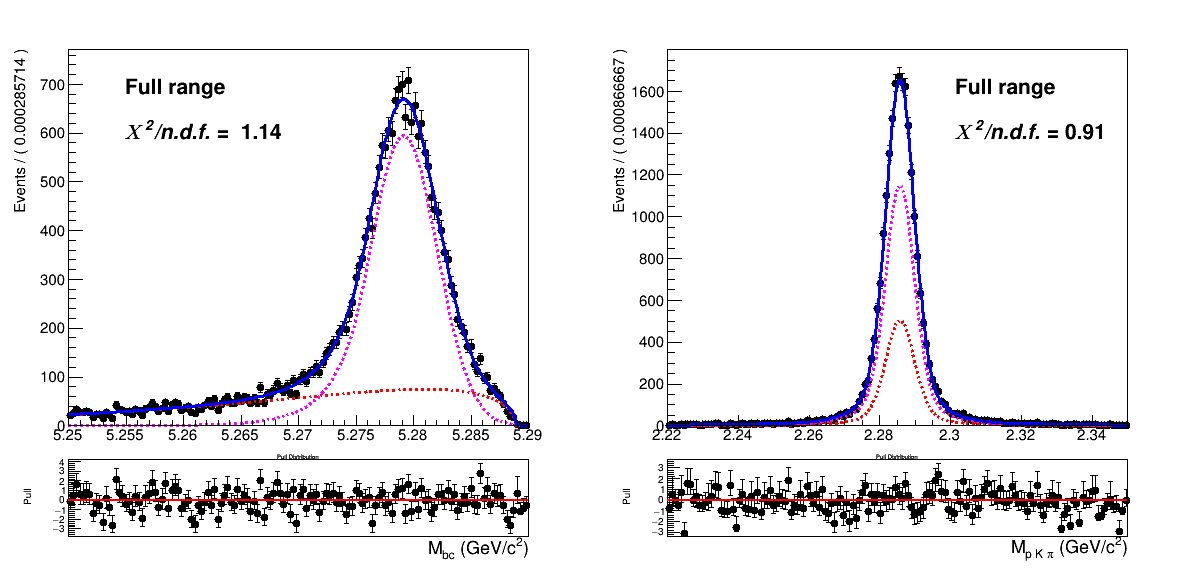
\includegraphics[width=0.7\textwidth]{04-SimultaneousFit/figs/5streams_TotalSignal_charged_corrLambdaC_2Dfit.png}}
\caption{Two dimensional fit of charged correlated total signal events in $M_{bc}$  and $M(p K \pi)$ }
\label{fig:5streams_TotalSignal_charged_corrLambdaC_2Dfit}
\end{figure}


    

\begin{figure}
\centering

{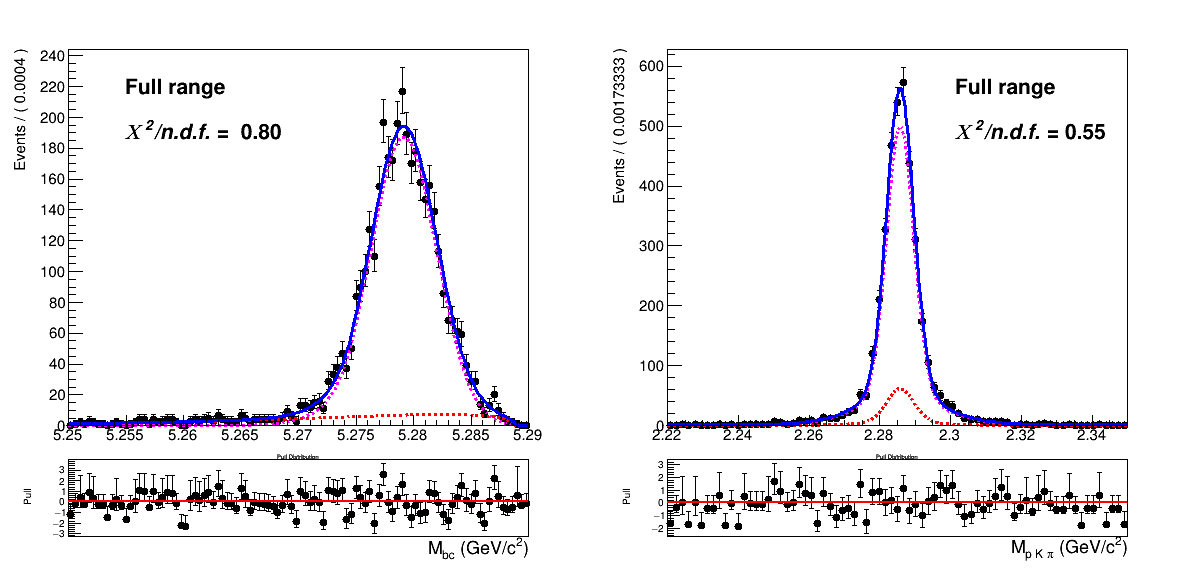
\includegraphics[width=0.7\textwidth]{04-SimultaneousFit/figs/stream12345_TotalSignal_charged_anticorrLambdaC_2Dfit.png}}
\caption{Two dimensional fit of charged anticorrelated total signal events in $M_{bc}$  and $M(p K \pi)$ }
\label{fig:5streams_TotalSignal_charged_anticorrLambdaC_2Dfit}
\end{figure}


\begin{figure}
\centering
{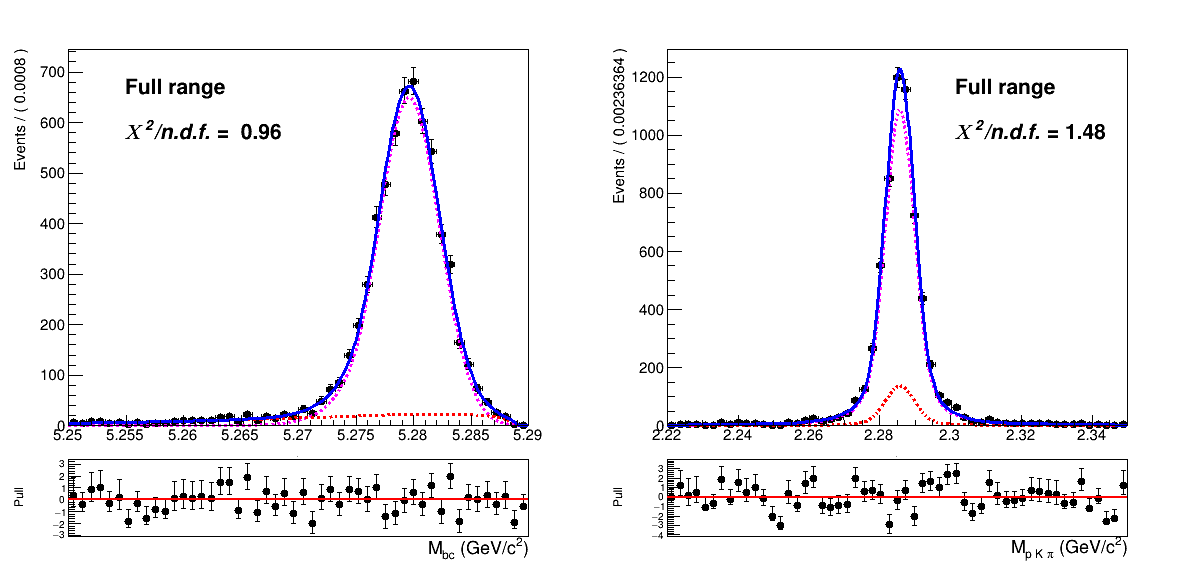
\includegraphics[width=0.7\textwidth]{04-SimultaneousFit/figs/NEWstream01234_TotalSignal_neutral_corrLambdaC_2Dfit.png}}
\caption{Two dimensional fit of neutral correlated total signal events in $M_{bc}$  and $M(p K \pi)$ }
\label{fig:5streams_TotalSignal_neutral_corrLambdaC_2Dfit}
\end{figure}

\begin{figure}
\centering
{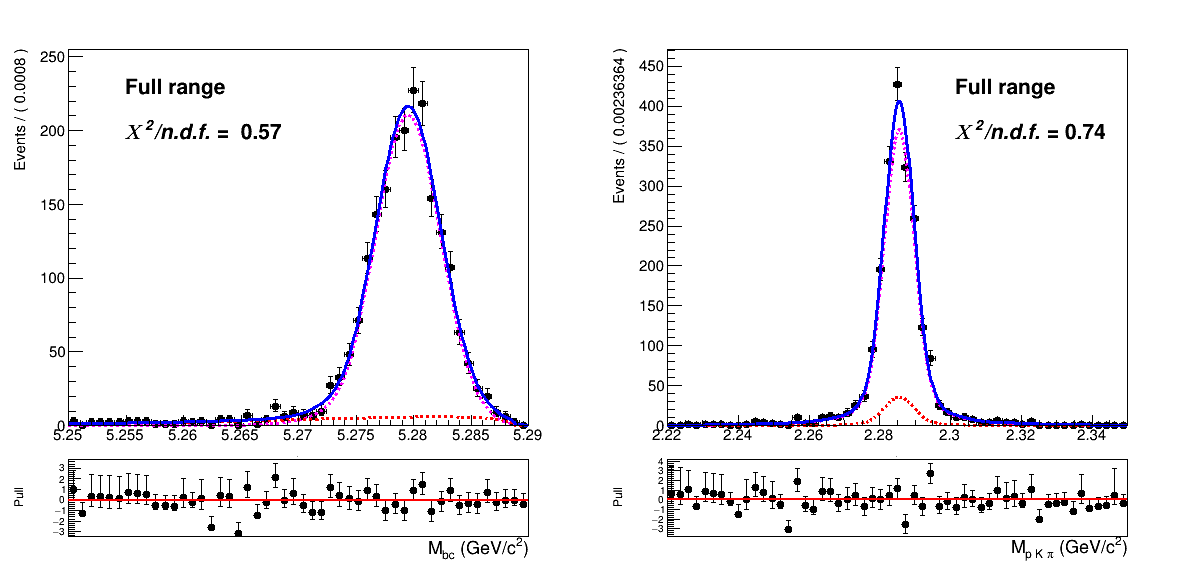
\includegraphics[width=0.7\textwidth]{04-SimultaneousFit/figs/NEWstream01234_TotalSignal_neutral_anticorrLambdaC_2Dfit.png}}
\caption{Two dimensional fit of neutral anticorrelated total signal events in $M_{bc}$  and $M(p K \pi)$ }
\label{fig:5streams_TotalSignal_neutral_anticorrLambdaC_2Dfit}
\end{figure}
\newpage
The 2D fits shown above are  performed on five streams of signal MC with a sum of the following probability density functions:
\vspace{0.2 cm}
 \begin{equation}
        P^{recSig}_{B,\Lambda_c}(M_{bc}, M(p K \pi)) = \Gamma_{CB}(M_{bc}) \times \rho_G(M(p K \pi))
    \label{eq:RecSigEq}
\end{equation} 
\begin{equation}
        P^{misSig}_{B,\Lambda_c}(M_{bc}, M(p K \pi)) = \Gamma_{ARG}(M_{bc}) \times \rho_G(M(p K \pi))
    \end{equation}  \label{eq:MisSigEq}

The first is used to fit the reconstructed signal and $\Gamma_{CB}(M_{bc})$ is a Crystal Ball function. The second is used to model the misreconstructed signal and $\Gamma_{ARG}(M_{bc})$ is an Argus function. In both cases a sum of three Gaussian functions $\rho_G(M(p K \pi))$ describes the mass of the $\Lambda_c$ baryon.  


As already said, only the events of reconstructed signal are considered as signal, while the misreconstructed signal is considered as background.

\subsection{Mbc peaking and flat background}

The background composed of $B\bar{B}$ events where no $\Lambda_c$ baryon  is produced, is flat in its invariant mass, but  can be distinguished in the following two categories:

\begin{itemize}
    \item peaking in $M_{bc}$ but not in $M$($p K \pi$)
    \item flat in both $M_{bc}$ and $M$($p K \pi$ )
\end{itemize}

as one can see in the following plots.

\begin{figure}
\centering
{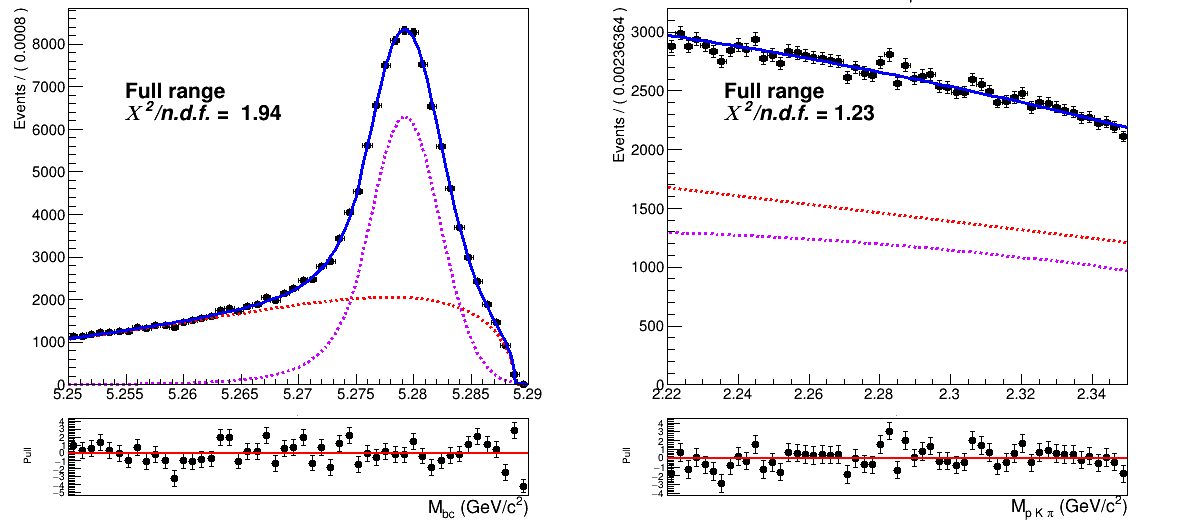
\includegraphics[width=0.7\textwidth]{04-SimultaneousFit/figs/stream01234_charged_corrLambdaC_TotalGeneric_2DFit_onlyArgus.png}}
\caption{Two dimensional fit of charged correlated $B\bar{B}$  events in $M_{bc}$  and $M(p K \pi)$ }
\label{fig:stream01234_charged_corrLambdaC_TotalGeneric_2DFit}
\end{figure}


\begin{figure}
\centering
{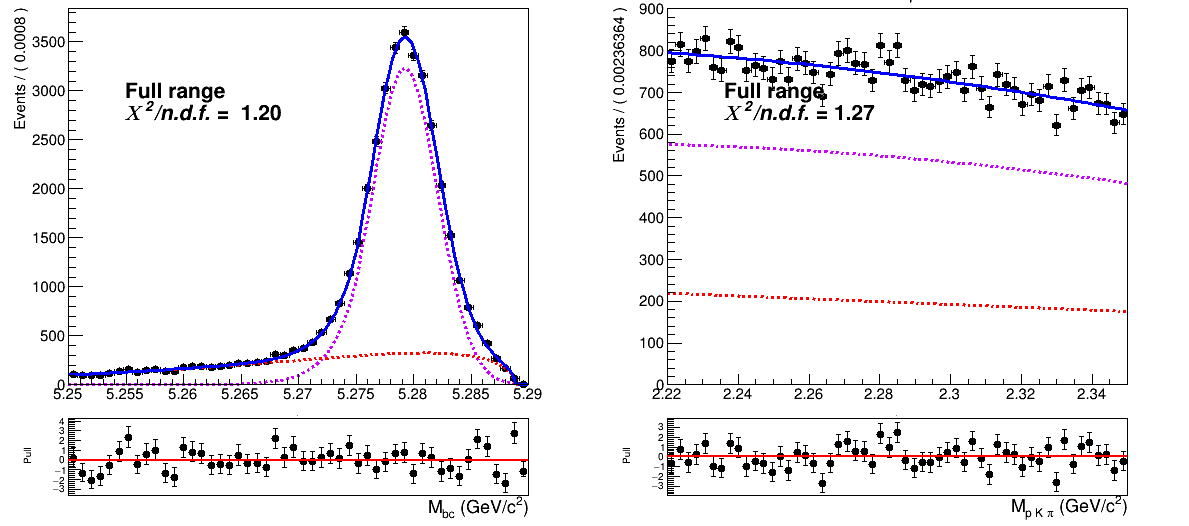
\includegraphics[width=0.7\textwidth]{04-SimultaneousFit/figs/stream12345_charged_anticorrLambdaC_TotalGeneric_2DFit_only_argus.png}}
\caption{Two dimensional fit of charged anticorrelated $B\bar{B}$  events in $M_{bc}$  and $M(p K \pi)$ }
\label{fig:stream12345_charged_anticorrLambdaC_TotalGeneric_2DFit}
\end{figure}

\begin{figure}
\centering
{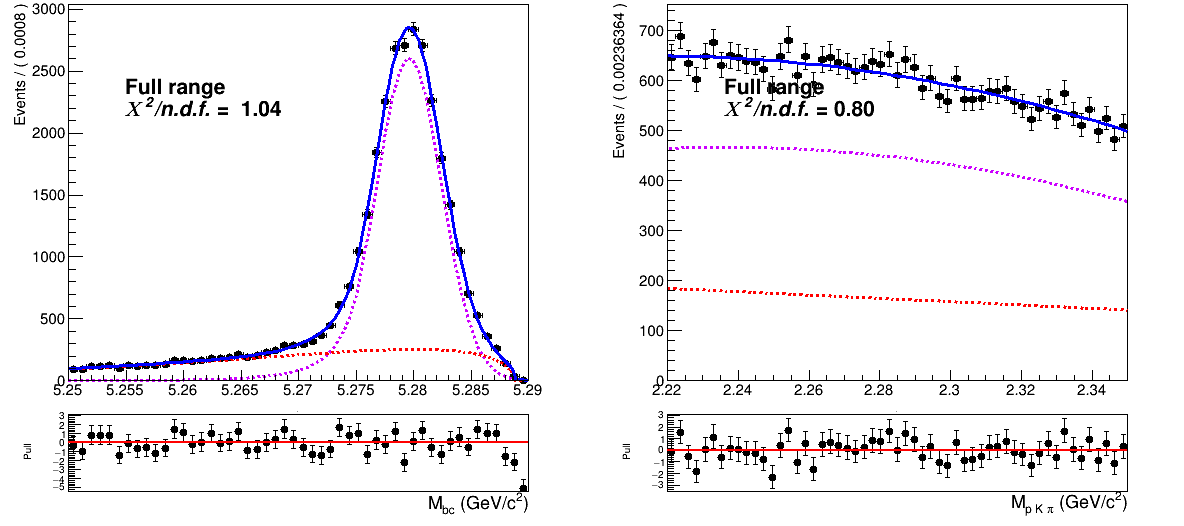
\includegraphics[width=0.7\textwidth]{04-SimultaneousFit/figs/stream01245_neutral_corrLambdaC_TotalGeneric_2DFit.png}}
\caption{Two dimensional fit of neutral correlated $B\bar{B}$  events in $M_{bc}$  and $M(p K \pi)$ }
\label{fig:stream01245_neutral_corrLambdaC_TotalGeneric_2DFit}
\end{figure}

\begin{figure}
\centering
{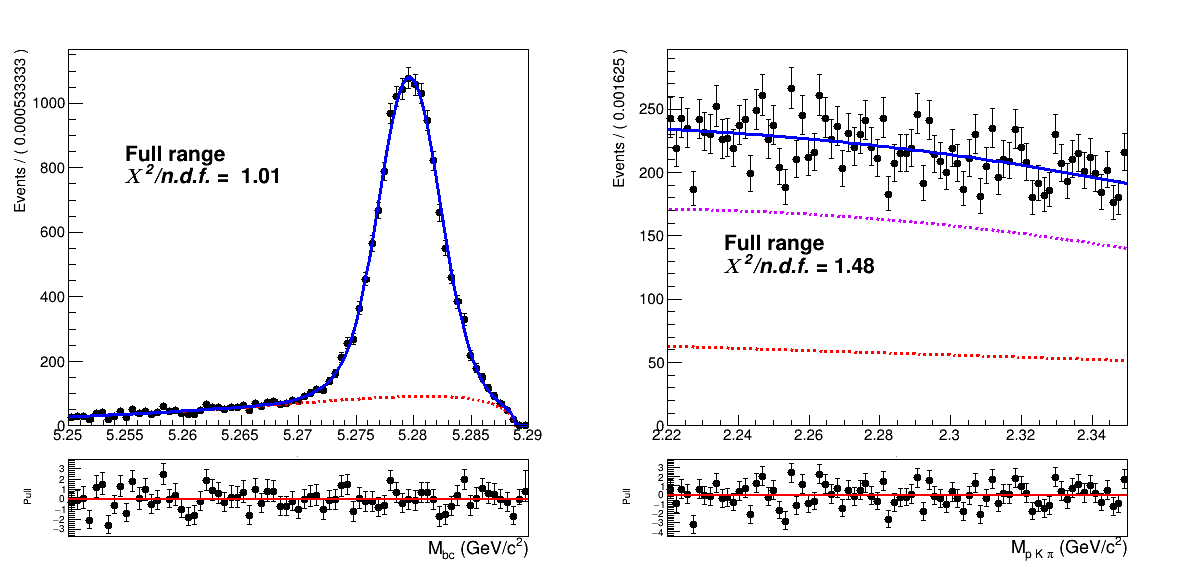
\includegraphics[width=0.7\textwidth]{04-SimultaneousFit/figs/stream01235_neutral_anticorrLambdaC_Generic_2DFit.png}}
\caption{Two dimensional fit of neutral anticorrelated $B\bar{B}$  events in $M_{bc}$  and $M(p K \pi)$ }
\label{fig:stream01235_neutral_anticorrLambdaC_Generic_2DFit}
\end{figure}


\newpage
This background presents a 
similar shape of the distribution in $M_{bc}$: the probability
density functions used for it are again a  Crystal Ball and an Argus. \\
The two types of background (peaking/flat in $M_{bc}$) are described by:
\begin{equation}
P^{peaking}_{B,\Lambda_c}(M_{bc}, M(p K \pi)) = \Gamma_{CB}(M_{bc})  \times \rho_{Cheb(a0,a 1)}(M(p K \pi))
\end{equation}

\begin{equation}
P^{flat}_{B,\Lambda_c}(M_{bc}, M(p K \pi)) =  \Gamma_{ARG}(M_{bc}) \times \rho_{Cheb(b0)}(M(p K \pi))
\end{equation}
\newline
%\vspace{0.5 cm}
where $\rho_{Cheb(a0,a 1)}(M(p K \pi))$ and $\rho_{Cheb(b0)}(M(p K \pi))$  represent a second order and first order Chebychev polynomial function respectively.

\subsection{Crossfeed background}
The contamination of misreconstructed $B^0 \rightarrow \Lambda_c$ events in the $B^+$ signal (and vice-versa) induces a background  peaking in $M(p K \pi)$, but it also slightly peaks near the $B$ meson mass, as one can see in Fig. \ref{fig:chargedBcorr_CrossfeedLambdaCpeak}
\newpage
\begin{figure}
\centering
{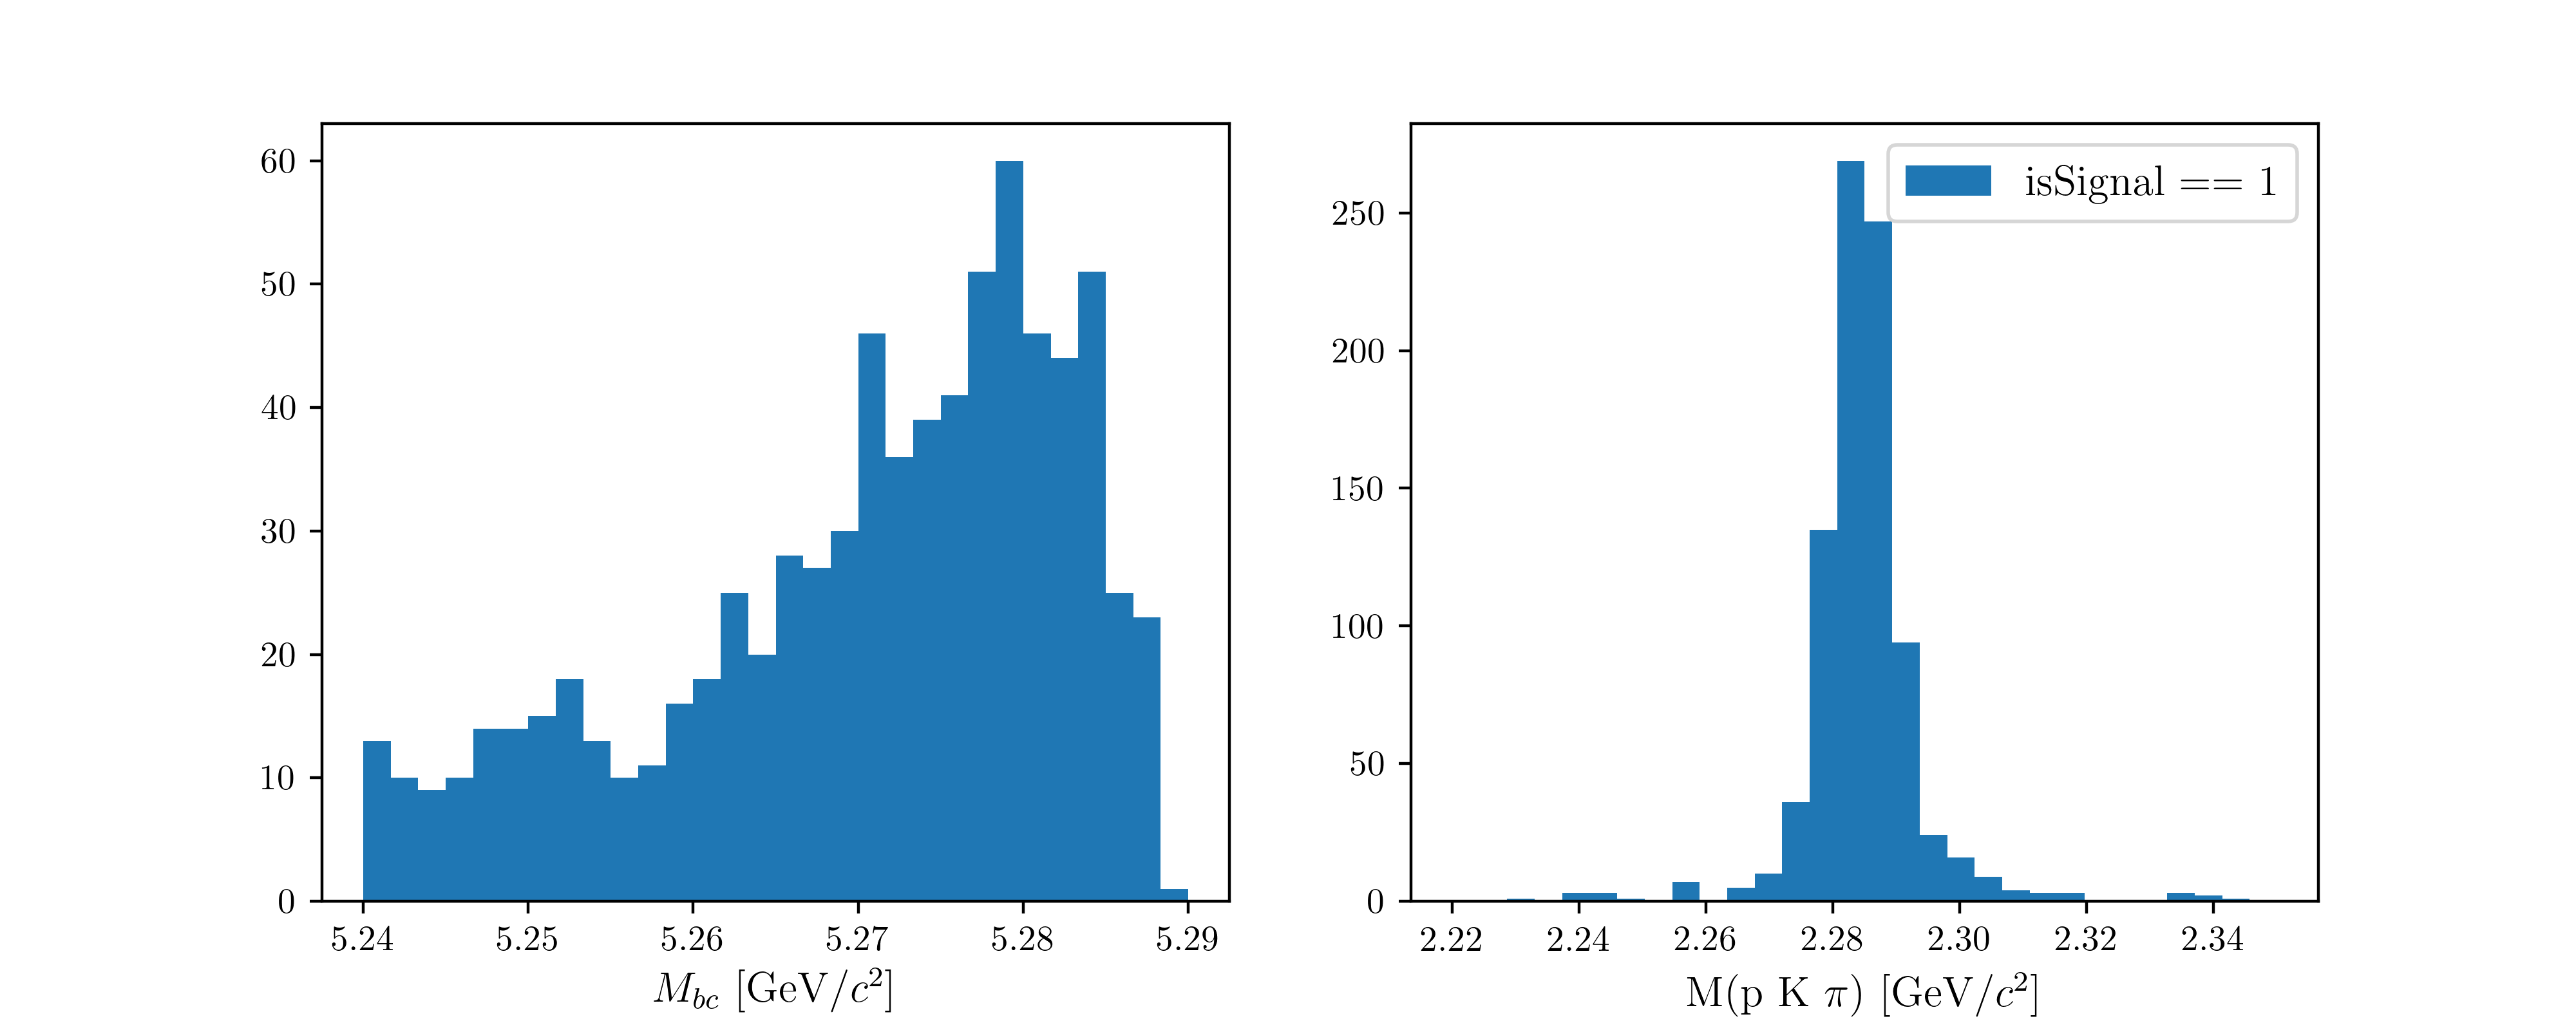
\includegraphics[width=0.8\textwidth]{04-SimultaneousFit/figs/chargedBcorr_CrossfeedLambdaCpeak.png}}
\caption{Crossfeed distribution in $M_{bc}$  and $M(p K \pi)$ }
\label{fig:chargedBcorr_CrossfeedLambdaCpeak}
\end{figure}


\begin{figure}
\centering
{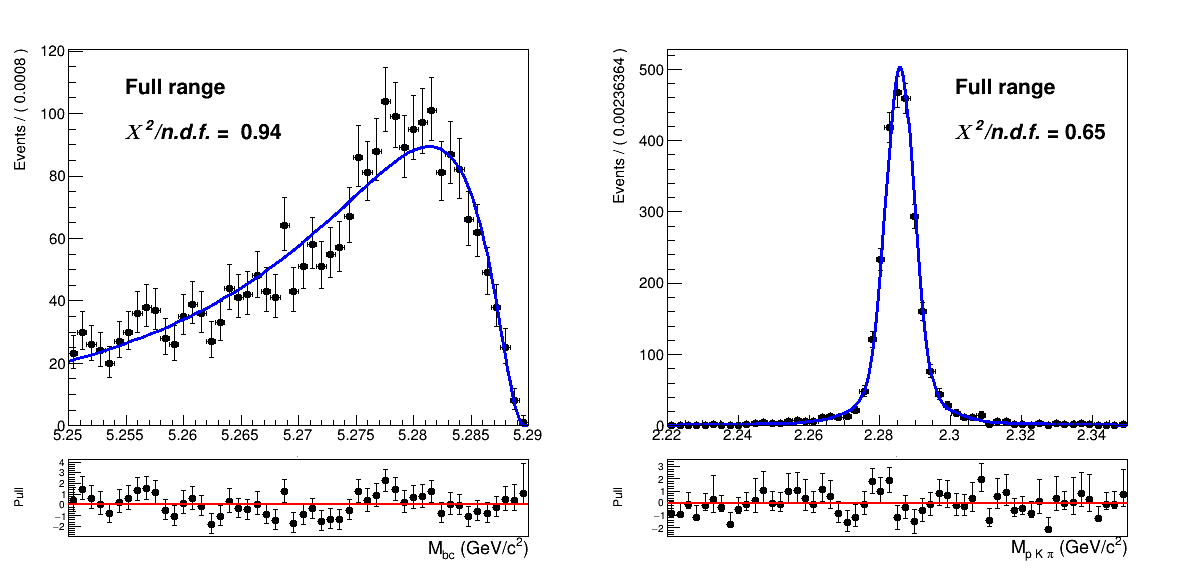
\includegraphics[width=0.7\textwidth]{04-SimultaneousFit/figs/streams01245_CrossfeedPeak_charged_corrLambdaC_2Dfit.png}}
\caption{Two dimensional fit of crossfeed events in charged correlated channel in $M_{bc}$  and $M(p K \pi)$ }
\label{fig:streams01245_CrossfeedPeak_charged_corrLambdaC_2Dfit}
\end{figure}


\begin{figure}
\centering
{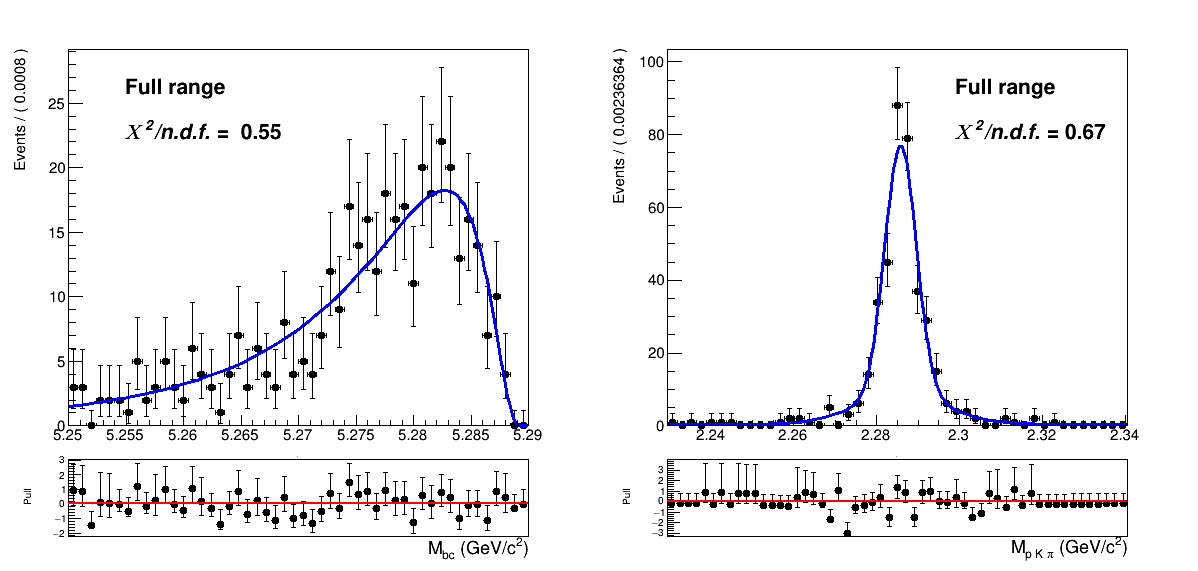
\includegraphics[width=0.7\textwidth]{04-SimultaneousFit/figs/streams01234_CrossfeedPeak_charged_anticorr_LambdaC_2Dfit.png}}
\caption{Two dimensional fit of crossfeed events in charged anticorrelated channel in $M_{bc}$  and $M(p K \pi)$ }
\label{fig:streams01234_CrossfeedPeak_charged_anticorr_LambdaC_2Dfit}
\end{figure}

\begin{figure}
\centering
{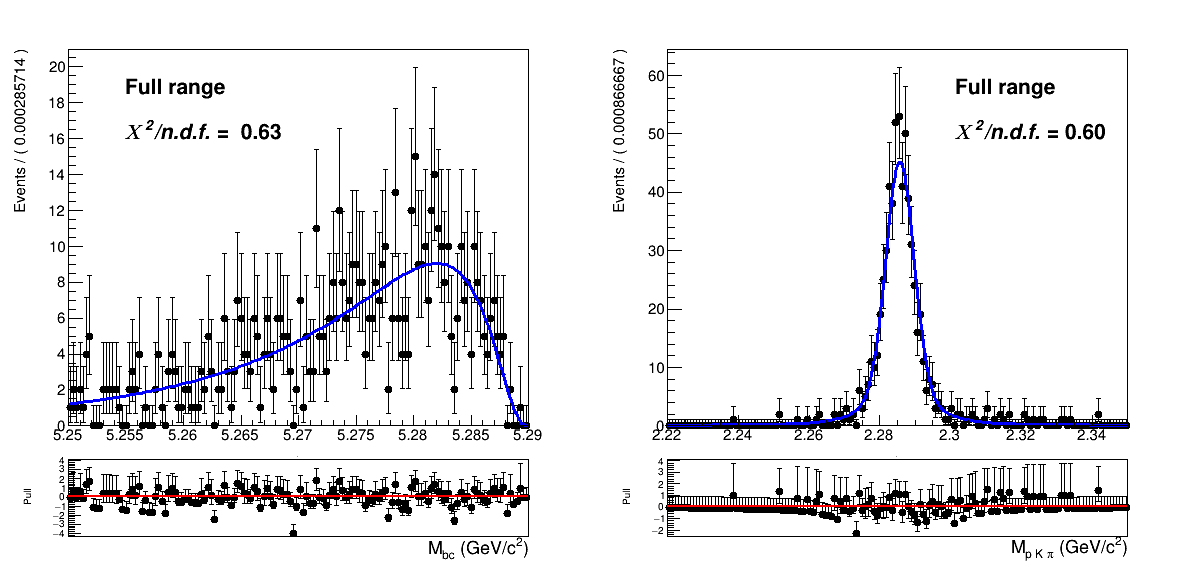
\includegraphics[width=0.7\textwidth]{04-SimultaneousFit/figs/streams01234_CrossfeedPeak_neutral_corrLambdaC_2Dfit.png}}
\caption{Two dimensional fit of crossfeed events in neutral correlated channel in $M_{bc}$  and $M(p K \pi)$ }
\label{fig:streams01234_CrossfeedPeak_neutral_corrLambdaC_2Dfit}
\end{figure}

\begin{figure}
\centering
{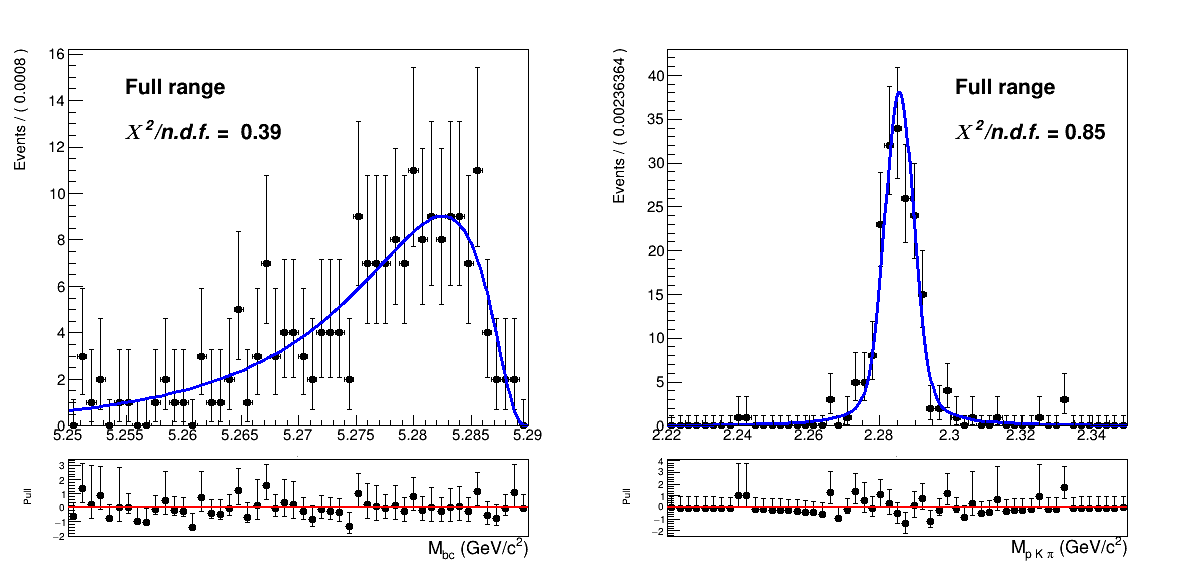
\includegraphics[width=0.7\textwidth]{04-SimultaneousFit/figs/stream12345_Crossfeed_neutral_anticorrLambdaC_2Dfit.png}}
\caption{Two dimensional fit of crossfeed events in neutral anticorrelated channel in $M_{bc}$  and $M(p K \pi)$ }
\label{fig:stream12345_Crossfeed_neutral_anticorrLambdaC_2Dfit}
\end{figure}

\newpage
The 2D fit shown above are  performed on five streams of signal MC with a sum of the following probability density function:
\vspace{0.2 cm}
 \begin{equation}
        P^{Crossfeed}_{B,\Lambda_c}(M_{bc}, M(p K \pi)) = \Gamma_{Novosibirsk}(M_{bc}) \times \rho_G(M(p K \pi))
    %\label{eq:}
\end{equation} 

where $\Gamma_{Novosibirsk}(M_{bc})$ is a Novosibirsk function and the mass of the $\Lambda_c$ baryon is described by the same sum of three Gaussian functions $\rho_G(M(p K \pi))$ as in Eq.\ref{eq:RecSigEq}.

\subsection{Continuum background}


 Besides the dataset recorded at the energy of the $\Upsilon(4S) $ resonance  ($E^{on-res}
_{CMS} = $ 10.58 GeV), the \textit{Belle} experiment recorded a sample of 89.4 $fb^{-1}$ at an energy 60 MeV below the nominal  $\Upsilon(4S) $ resonance ($E^{off-res}_{CMS} = $ 10.52 GeV). The dataset allows to check for an appropriate modeling of the continuum MC simulation. %, by comparing the off-resonance data with the MC expectation for the continuum background. 
Using the official tables \newline ( \url{https://belle.kek.jp/secured/nbb/nbb.html}) the off-resonance sample is scaled by 

\begin{equation}
    \frac{\mathcal{L}^{on-res}}{\mathcal{L}^{off-res}} \left( \frac{E^{off-res}_{CMS}}{E^{on-res}_{CMS}}\right)^2
\label{eq:off-resScaling}
\end{equation}


\noindent taking into account the difference in luminosity and in $E_{CMS}$ (Energy in center of mass system).


\begin{figure}[h!]
%\centering
{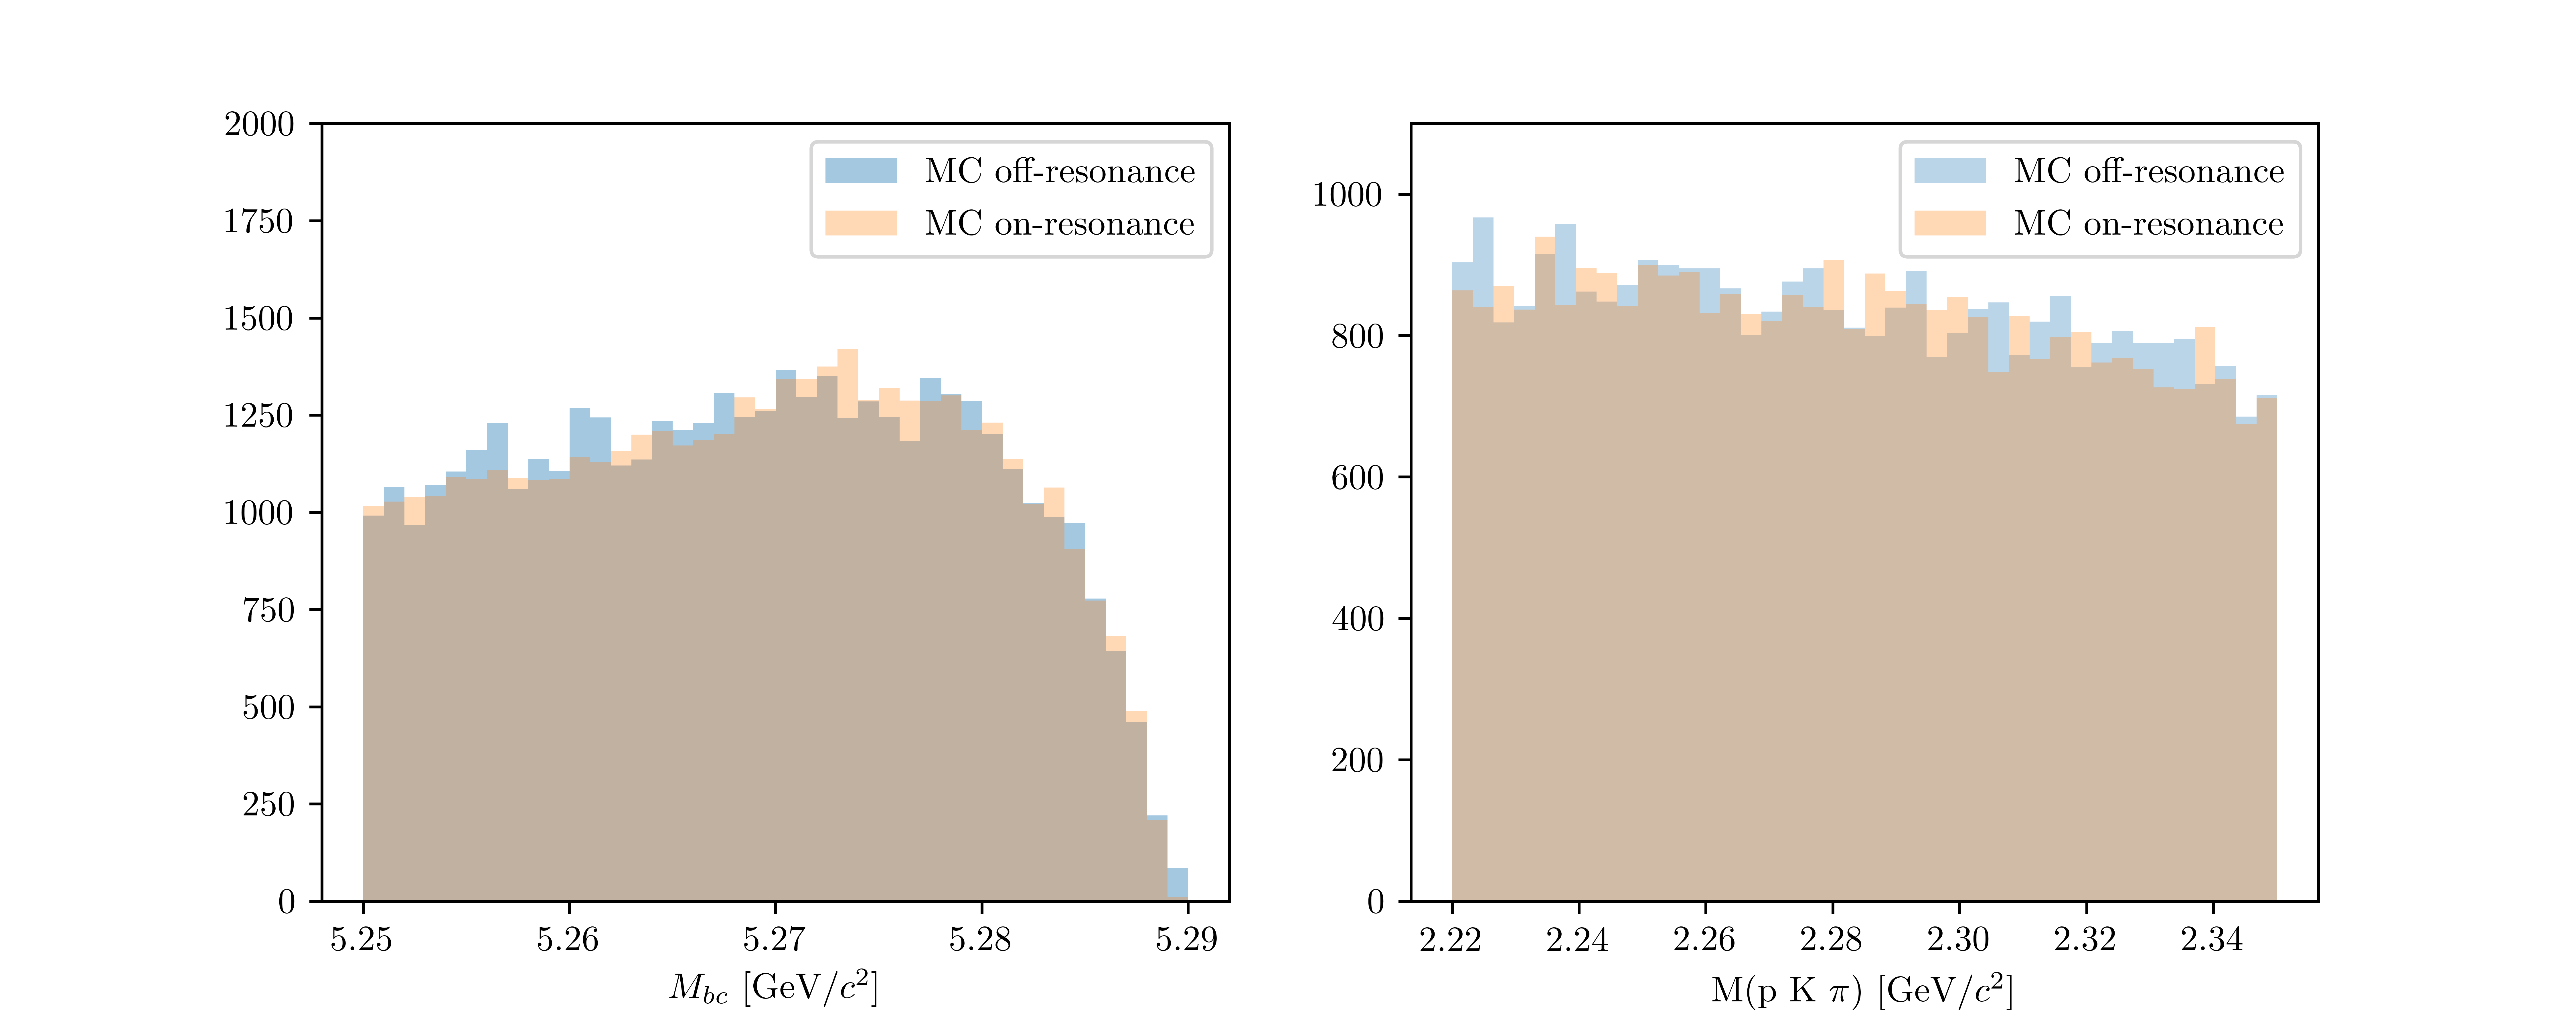
\includegraphics[width=1.05\textwidth]{04-SimultaneousFit/figs/MbcInvM_MC_on_off-resonance_comparison.png}}
\caption{$M_{bc}$ and $M(p K \pi)$ comparison between  on-/off-resonance (scaled) Monte Carlo simulated continuum. The scaling is applied according to \cref{eq:off-resScaling} and shifting the $M_{bc}$ distribution by $E^{on-res}_{CMS} - E^{off-res}_{CMS}$. }
\label{fig:MbcInvM_MC_on_off-resonance_comparison}
\end{figure} 

\noindent The plot in Fig.\ref{fig:MbcInvM_MC_on_off-resonance_comparison} shows the $M_{bc}$ and $M(p K \pi)$ distributions in the MC on-/off-resonance continuum after the scaling\footnote{it is obtained with the MC off-resonance sample being composed of 6 streams: the total amount is normalized}.

Ideally, provided that there's a good agreement between MC and data for the off-resonance sample and also between the MC  on-/off-resonance continuum after the scaling, one could directly use the scaled off-resonance data to describe the continuum background in the fit on data. There are two reasons that prevent this very straightforward approach:
\begin{itemize}

\item First, since the off-resonance MC (and data) present very low statistics (Fig. \ref{fig:off-resData_charged_corrLambdaC_InvM} shows the  $\Lambda_c$ 
invariant mass in off-resonance data), scaling them with all the applied selection cuts would cause the PDF describing the continuum to be very much affected by statistical fluctuations. 
\item Secondly, the $B$ meson candidates are reconstructed in both on-resonance and off-resonance events for values of $M_{bc} \geq 5.22 $ GeV/c$^2$, but the $E_{CMS}$ differs: there can be effects of correlations between the applied \textit{SignalProbability} cut and the $M_{bc}$ variable that one needs to take into account. %This effects on the $M_{bc}$ are carefully studied in the analysis of the control sample. 
\end{itemize}


\begin{figure}
\centering
\subcaptionbox{\label{fig:off-resData_charged_corrLambdaC_InvM}}
{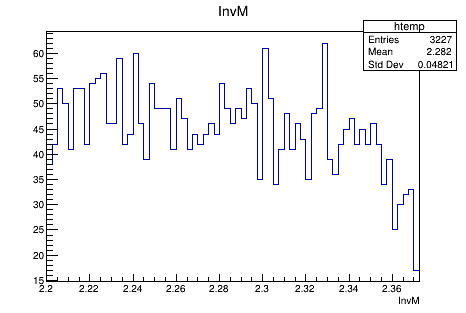
\includegraphics[width=.45\textwidth]{04-SimultaneousFit/figs/chargedCorrLambdaC_off-resData.png}}\quad
\subcaptionbox{\label{fig:off-resData_charged_corrLambdaC_InvM_woCS}}
{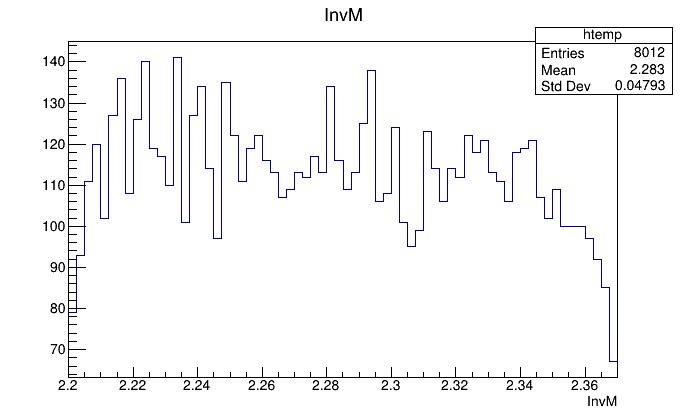
\includegraphics[width=.48\textwidth]{04-SimultaneousFit/figs/chargedCorrLambdaC_off-resData_woCScuts.png}} \quad
\caption{On the left: $\Lambda_c$ invariant mass in off-resonance data (all nominal cuts applied). On the right: $\Lambda_c$ invariant mass in off-resonance data after the continuum suppression cut removal.}
\end{figure}


\begin{figure}[H]
%\centering
{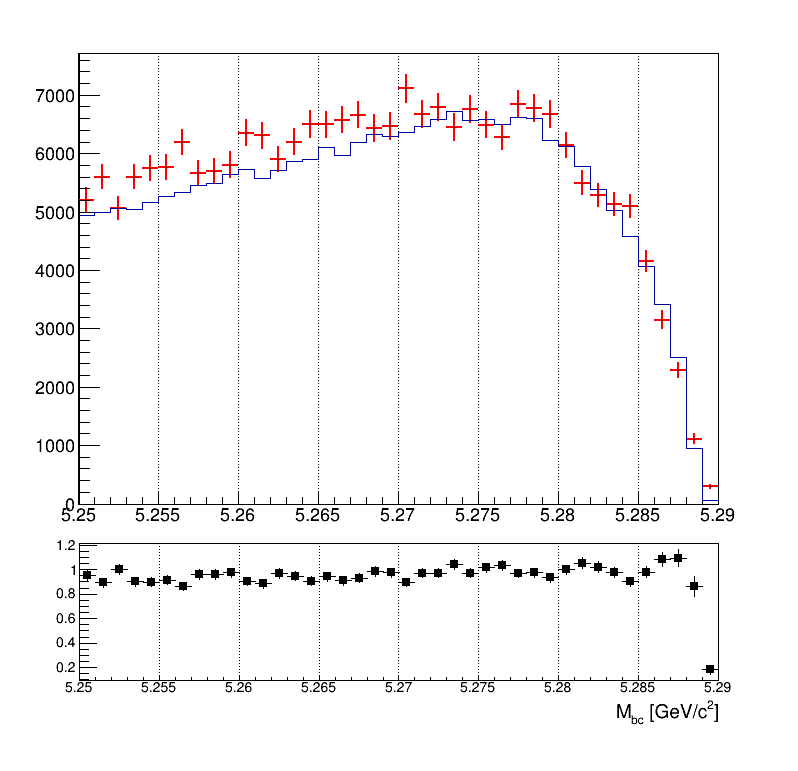
\includegraphics[width=0.5\textwidth]{04-SimultaneousFit/figs/stream01234_Mbc_continuumRescaling.png}}
\caption{$M_{bc}$ distributions of the MC (scaled) off-resonance sample (in red) and on-resonance (in blue) using 5 streams statistics and all nominal selection cuts applied.}
\label{fig:charged_corrLambdaC_Mbc_on_offResScaled}
\end{figure}

In Fig. \ref{fig:charged_corrLambdaC_Mbc_on_offResScaled} one can notice some discrepancy in the shapes, apart from the not negligible statistical fluctuations in the (scaled) off-resonance distribution.  



\newpage


\begin{figure}
\centering
\subcaptionbox{\label{fig:onRes_offResScaledMbc_corrLambdaC}}
{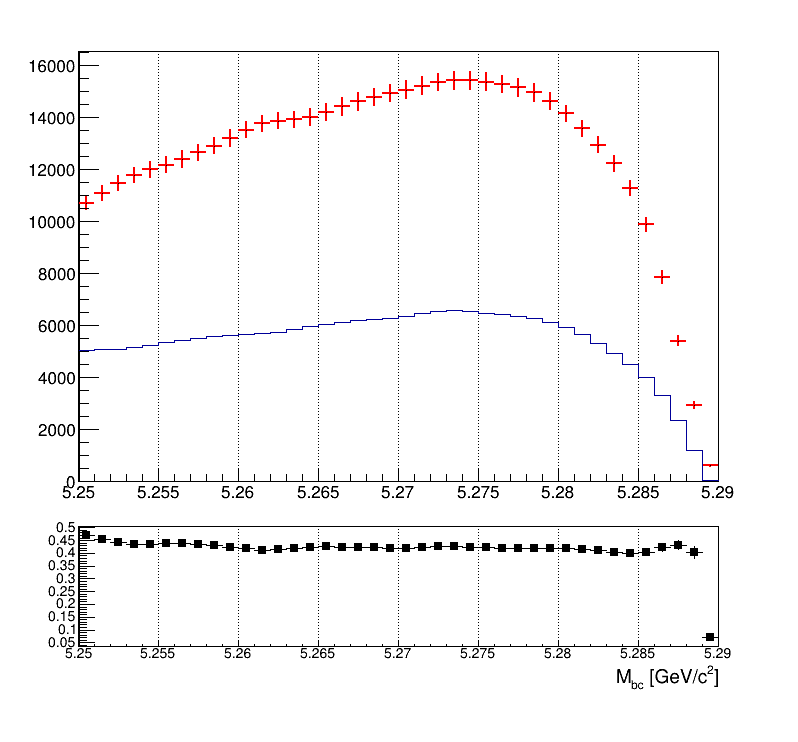
\includegraphics[width=.46\textwidth]{04-SimultaneousFit/figs/stream01235_charged_corrLambdaC_woCScuts_Mbc_scaling.png}} \quad
\subcaptionbox{\label{fig:Mbc_scaled_bin_correctedOffResContinuum}}
{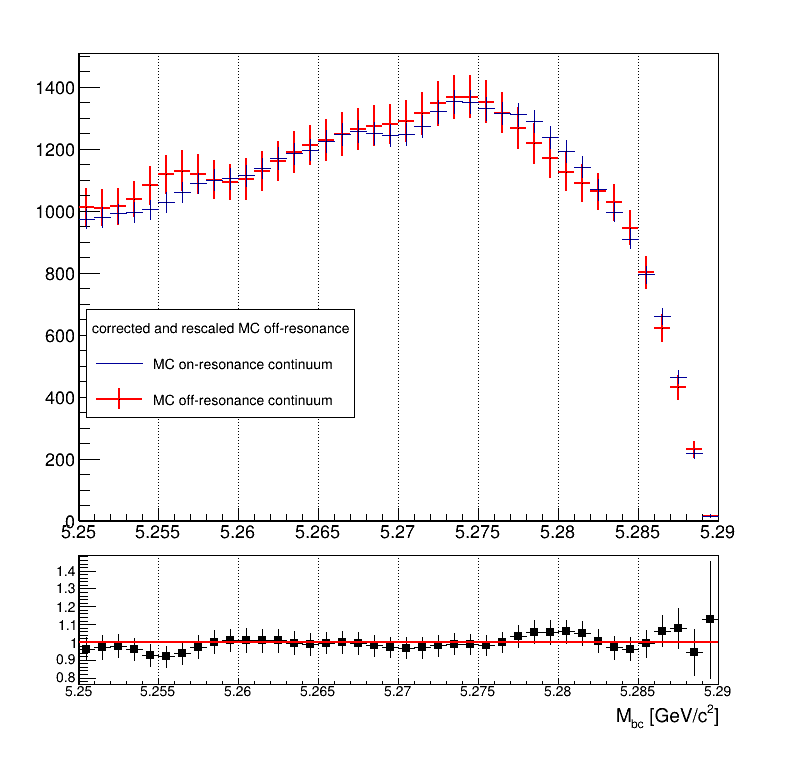
\includegraphics[width=.44\textwidth]{04-SimultaneousFit/figs/MC_on_off_resonance_stream4_continuum_2D_Mbc_corrected.png}} \quad
\caption{On the left: $M_{bc}$ distributions of the MC off-resonance sample without continuum suppression and the MC continuum sample with applied continuum suppression. On the right: $M_{bc}$ distributions of the corrected scaled MC off-resonance and on-resonance MC continuum.}
\end{figure}


The procedure adopted to obtain the PDF describing the continuum background  $M_{bc}$ distribution is the following:
\begin{itemize}

\item 5 streams of off-resonance MC were scaled according to \cref{eq:off-resScaling} without continuum suppression being applied and compared to the distribution of 5 streams of on-resonance continuum
\item From a ratio plot, like the one in Fig. \ref{fig:onRes_offResScaledMbc_corrLambdaC}, the bin-correction is obtained to correct the off-resonance data in the scaling procedure.
To obtain the shape that can describe the continuum background  $M_{bc}$ distribution on data the continuum suppression is not applied on the off-resonance continuum sample, in order to acquire more statistics. 
\end{itemize}

\noindent This procedure is first tested on an independent MC sample (see Fig. \ref{fig:Mbc_scaled_bin_correctedOffResContinuum} ) to check the result on simulated data before applying it on data.



\begin{figure}[H]
\centering
\subcaptionbox{\label{fig:corrLambdaC_OffResonance_w_wo_CS_comparison_5streams}}
{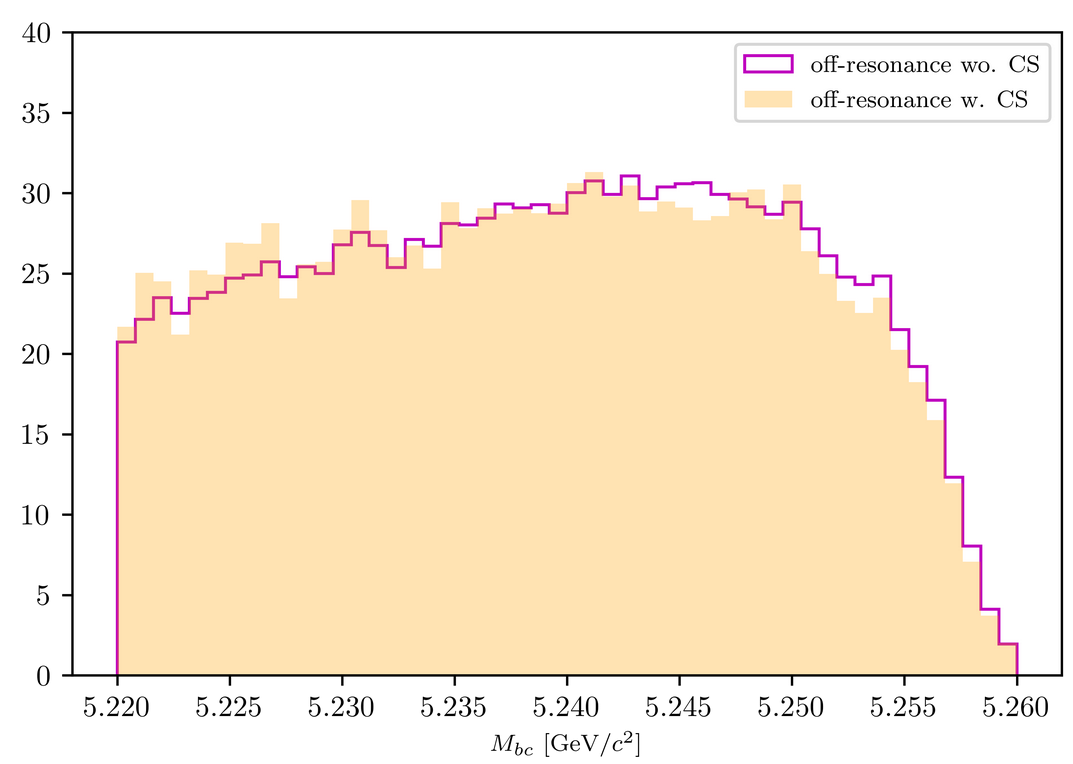
\includegraphics[width=.65\textwidth]{04-SimultaneousFit/figs/corrLambdaC_OffResonance_w_wo_CS_comparison_5streams.png}} 
\subcaptionbox{\label{fig:corrLambdaC_OffResonance_w_wo_CS_comparison_Data}}
{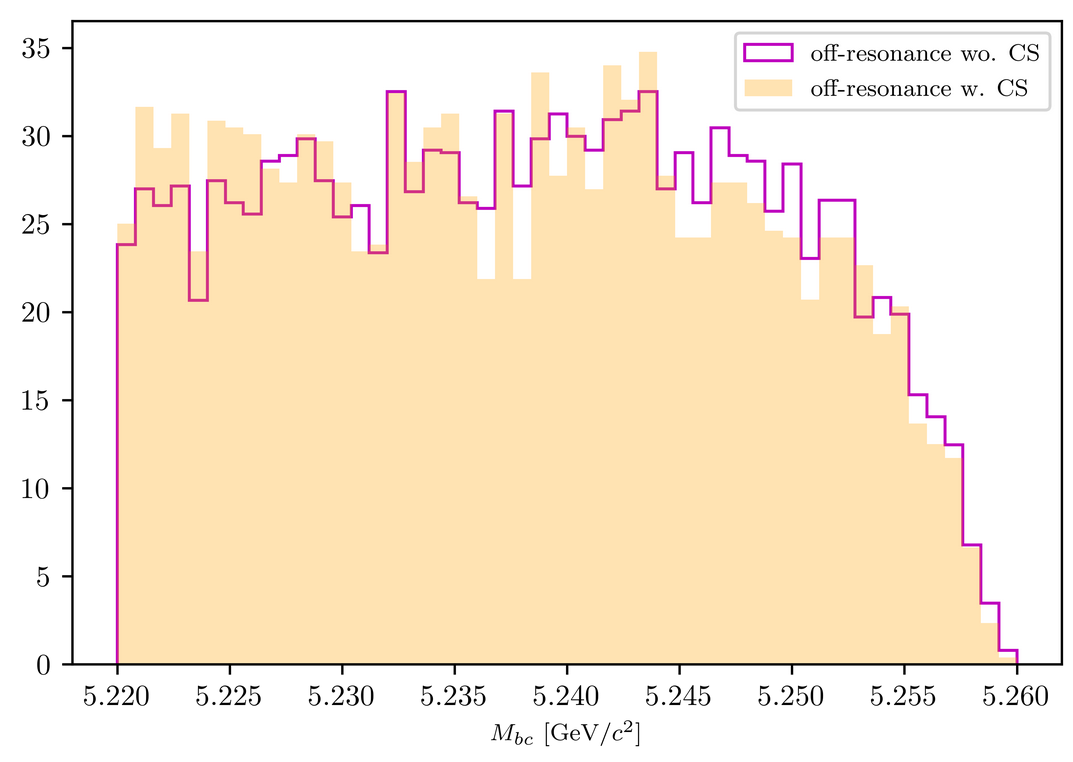
\includegraphics[width=.65\textwidth]{04-SimultaneousFit/figs/corrLambdaC_OffResonance_w_wo_CS_comparison_Data.png}} 
\caption{Above: $M_{bc}$ distributions of the MC off-resonance sample (5 streams) with and without continuum suppression. Below: $M_{bc}$ distributions on data with and without continuum suppression.}
\end{figure}




\noindent The validity of the method relies on the fact that the difference between  on-/off-resonance continuum events are well modeled in MC and that the shape of the $M_{bc}$ distribution doesn't change significantly when removing the continuum suppression cut both on MC and data (as one can see from Figures \ref{fig:corrLambdaC_OffResonance_w_wo_CS_comparison_5streams} - \ref{fig:corrLambdaC_OffResonance_w_wo_CS_comparison_Data}).\\
Additionally, the continuum suppression cut efficiency should be the same in data and MC in order to have the correct scaling on data with the above mentioned method. Fig. \ref{fig:R2_MC-Data_off_resonance_distributions} shows the distribution of the $foxWolframR2$ variable in off-resonance MC and data. The slight shift visible in data can cause a different impact on data in terms of rejected continuum background when applying the $foxWolframR2 < 0.3$ cut. It is found to reject about 60$\%$ of the continuum background in data, whereas it rejects 55$\%$ of the continuum background in MC ( 56$\%$ in on-resonance MC). Therefore in data one can expect about 2.25$\%$ less continuum background events. This discrepancy is not statistically significant (the statistical uncertainty for the continuum background events is of the level of $\sim 1\%$),  a simple correction to the number of events can be applied on data and its possible systematics can be then taken into account.



\begin{figure}
\centering
{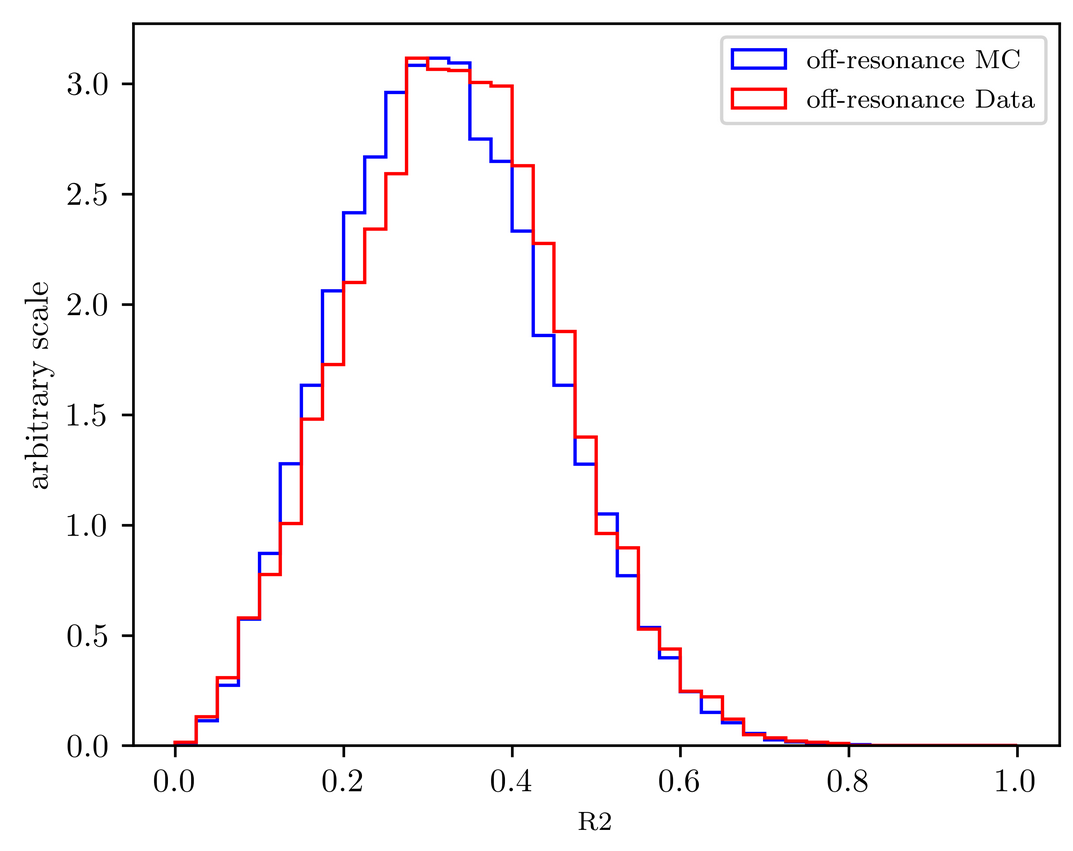
\includegraphics[width=0.5\textwidth]{04-SimultaneousFit/figs/R2_MC-Data_off_resonance_distributions.png}}
\caption{Distributions of variable $foxWolframR2$ in off-resonance MC and data.}
\label{fig:R2_MC-Data_off_resonance_distributions}
\end{figure}

\noindent  The obtained distribution can be then fitted with a Novosibirsk function (see Fig. \ref{fig:charged_corrLambdaC_Mbc_continuumMC_fit}). \\
This is the procedure which can be then applied on the off-resonance data to obtain the $M_{bc}$ shape describing the continuum background in data.
\begin{figure}
\centering
{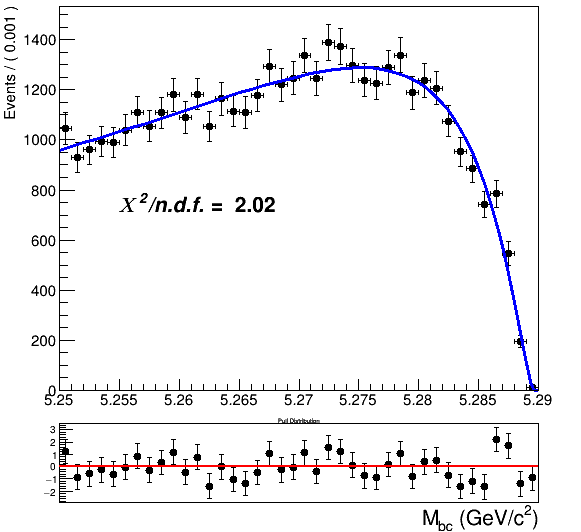
\includegraphics[width=0.43\textwidth]{04-SimultaneousFit/figs/stream5_rescaledMbc_40binsHist.png}}
\caption{Fit of the $M_{bc}$ distribution   MC (scaled) off-resonance continuum (one stream).}
\label{fig:charged_corrLambdaC_Mbc_continuumMC_fit}
\end{figure}

In the $\Lambda_c$ invariant mass one doesn't expect correlation effects, but nevertheless there can be differences due to the limited statistics of the off-resonance sample. 
In fact, in the case of on-resonance MC for the charged correlated decays some events in which  $\Lambda_c$ candidates survive nominal selection cuts are visible and can be described with a small Gaussian on the top of the flat background (Fig.\ref{fig:onRes_InvM_corrLambdaC}). Due to the low statistics one cannot see a similar peak in the off-resonance sample (the Fig.\ref{fig:5streams_offRes_InvM_corrLambdaC} shows a 5 streams statistics).

The shape describing the $\Lambda_c$ invariant mass in the case of charged correlated decays is obtained from the simulated on-resonance continuum, again using 5 streams statistics (see Fig. \ref{fig:onRes_InvM_corrLambdaC} ). In the other cases no peak is visible and therefore also the $\Lambda_c$ invariant mass shape is obtained from 5 streams of off-resonance events.


\begin{figure}
\centering
\subcaptionbox{\label{fig:onRes_InvM_corrLambdaC}}
{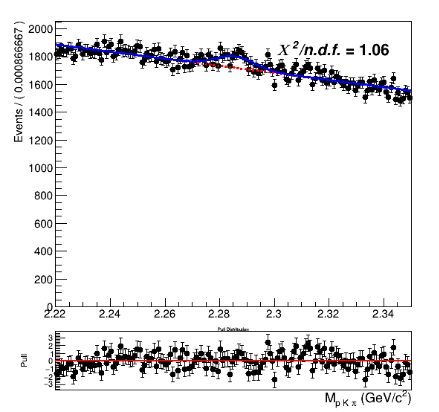
\includegraphics[width=.45\textwidth]{04-SimultaneousFit/figs/onRes_InvM_corrLambdaC.png}} 
\subcaptionbox{\label{fig:5streams_offRes_InvM_corrLambdaC}}
{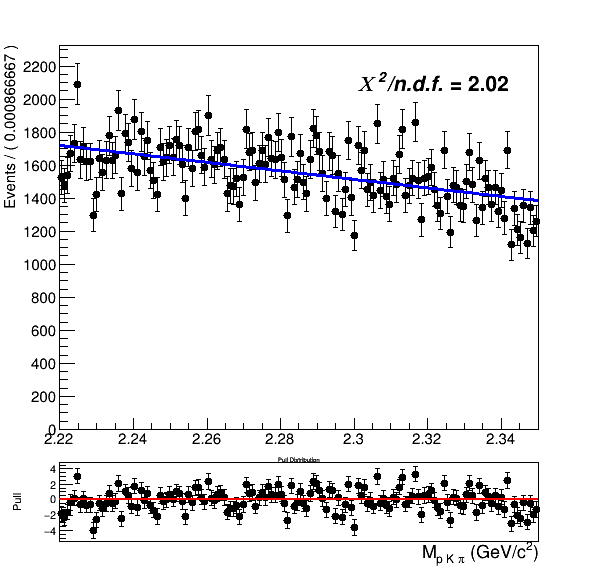
\includegraphics[width=.46\textwidth]{04-SimultaneousFit/figs/5streams_Off_resonanceRescaledContinuum_charged_corrLambdaC_oneGaussianInvMfit.png}} 
\caption{Comparison between 5 streams of MC on-resonance continuum \ref{fig:onRes_InvM_corrLambdaC}) and off-resonance (scaled) continuum in $M(p K \pi)$ (\ref{fig:5streams_offRes_InvM_corrLambdaC}).}
%\label{}
\end{figure}
%\newpage

Finally, it is possible to examine the validity of the whole procedure on the independent stream. 
Fig. \ref{fig:stream3corrLambddaC_total_continuum_2DFit} - \ref{fig:stream0_neutral_anticorrLambddaC_total_continuum_2DFit} show the $M_{bc}$, $M(p K \pi)$ projections of the overlayed two dimensional PDFs  obtained with the above described procedure.\\
The 2D PDF used for Fig. \ref{fig:stream3corrLambddaC_total_continuum_2DFit} can be written as: \\
 \vspace{0.2 cm}

$P^{Continuum}_{B,\Lambda_c}(M_{bc}, M(p K \pi)) = \Gamma_{Nov}(M_{bc}) \times [\rho_{Cheb1}(M(p K \pi) + \rho_{G}(M(p K \pi))]$\\
\vspace{0.2 cm}

where, as already anticipated, the invariant mass is described by a sum of a first order Chebychev polynomial and the peak by the same triple Gaussian PDF adopted for the signal. The  2D PDF used for Fig. \ref{fig:stream0_anticorrLambddaC_total_continuum_2DFit_Novosibirsk} and Fig. \ref{fig:stream0_neutral_corrLambddaC_total_continuum_2DFit_Novosibirsk} differ only in the invariant mass, not having the triple gaussian. Whereas the 2D PDF used for Fig. \ref{fig:stream0_neutral_anticorrLambddaC_total_continuum_2DFit} can be written as: \\
 \vspace{0.2 cm}

$P^{Continuum}_{B,\Lambda_c}(M_{bc}, M(p K \pi)) = \Gamma_{Argus}(M_{bc}) \times [\rho_{Cheb1}(M(p K \pi) ]$\\
\vspace{0.2 cm}

since the distribution in $M_{bc}$ can be better described by an Argus.
\begin{figure}
%\centering
{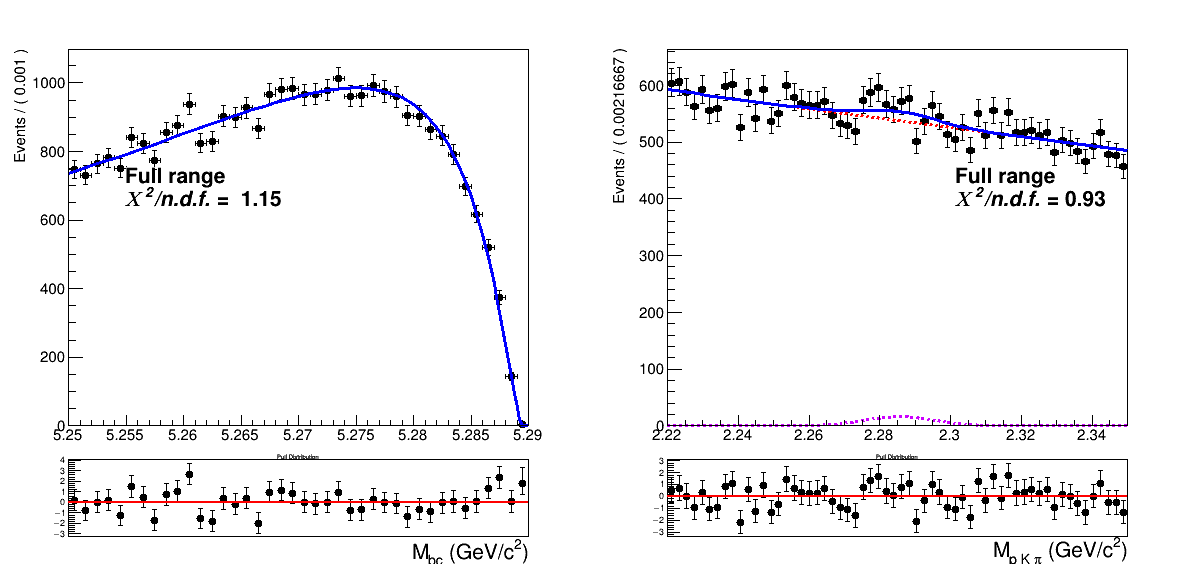
\includegraphics[width=0.85\textwidth]{04-SimultaneousFit/figs/stream3corrLambddaC_total_continuum_2DFit.png}}
\caption{Two dimensional fit of charged correlated  continuum events (one stream).}
\label{fig:stream3corrLambddaC_total_continuum_2DFit}
\end{figure}


\begin{figure}
%\centering
{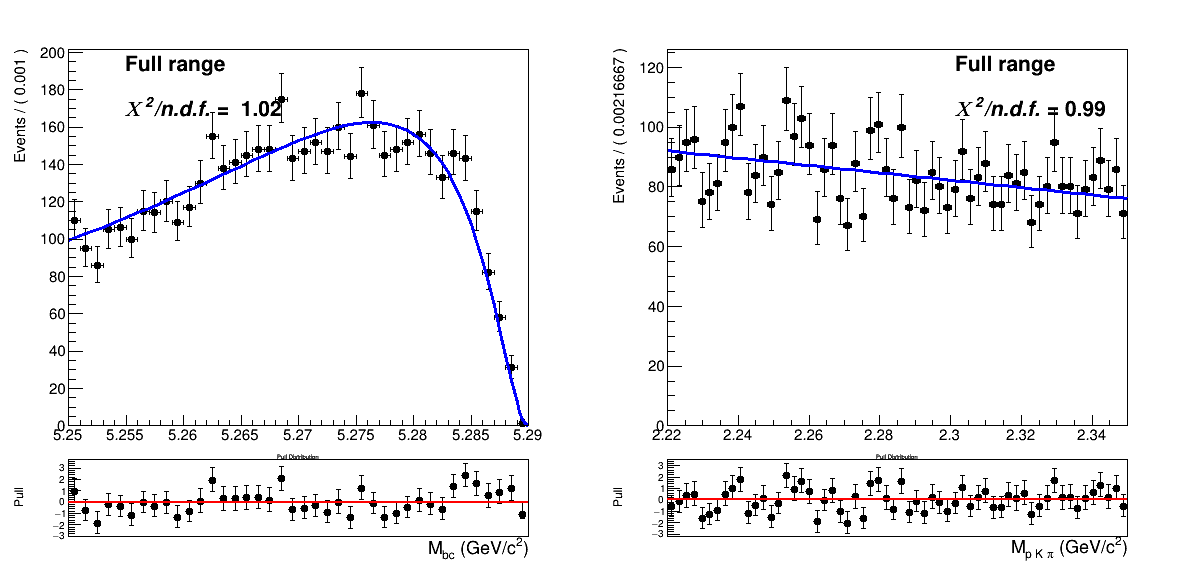
\includegraphics[width=0.85\textwidth]{04-SimultaneousFit/figs/stream0_anticorrLambddaC_total_continuum_2DFit_Novosibirsk.png}}
\caption{Two dimensional fit of charged anticorrelated continuum events (one stream).}
\label{fig:stream0_anticorrLambddaC_total_continuum_2DFit_Novosibirsk}
\end{figure}

\begin{figure}
%\centering
{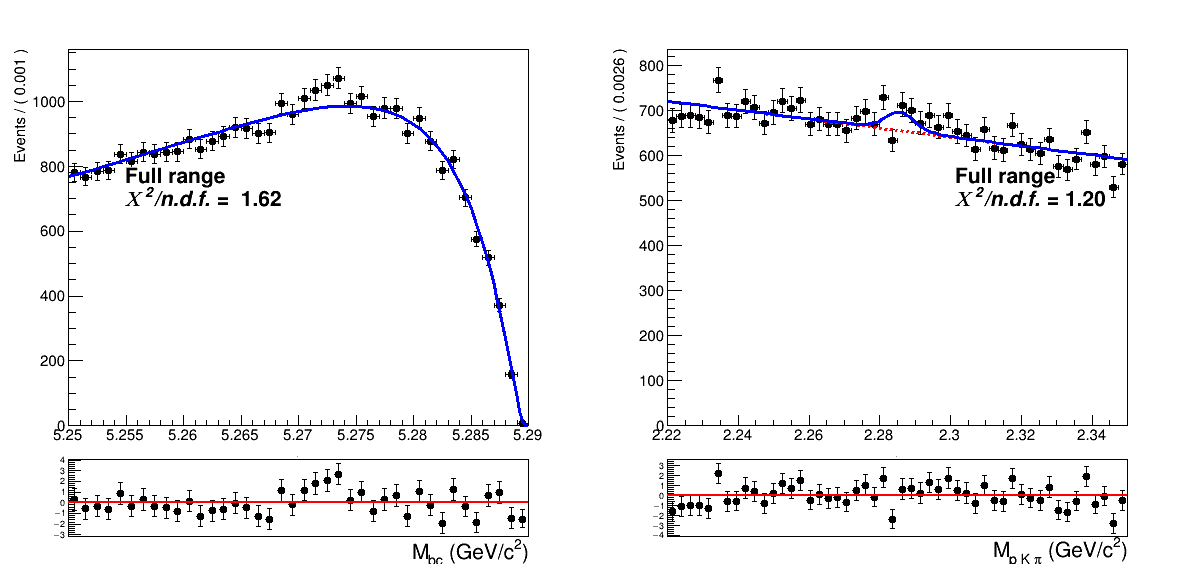
\includegraphics[width=0.85\textwidth]{04-SimultaneousFit/figs/stream0corrLambddaC_total_continuum_2DFit.png}}
\caption{Two dimensional fit of  continuum events (one stream).}
\label{fig:stream0_neutral_corrLambddaC_total_continuum_2DFit_Novosibirsk}
\end{figure}

\begin{figure}
%\centering
{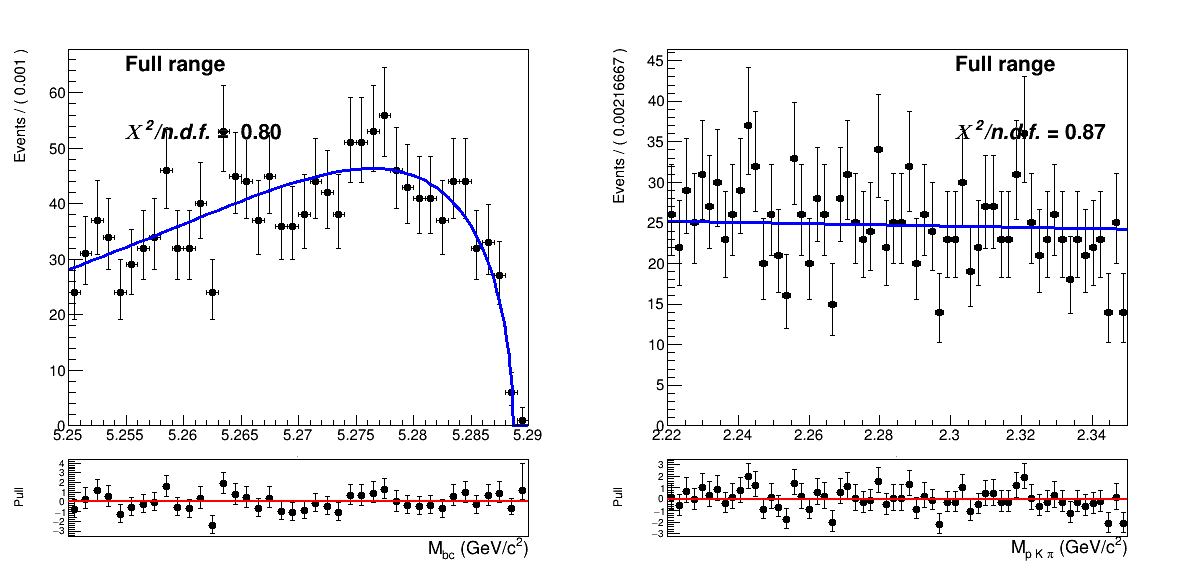
\includegraphics[width=0.85\textwidth]{04-SimultaneousFit/figs/stream0_anticorrLambddaC_total_continuum_2DFit_Argus.png}}
\caption{Two dimensional fit of  continuum events (one stream).}
\label{fig:stream0_neutral_anticorrLambddaC_total_continuum_2DFit}
\end{figure}


\newpage

\section{Two dimensional fit on Monte Carlo}\label{MC2D_Fit}

A total of six independent streams were used to construct/validate the fit model: each time five streams were 
used to construct the already discussed PDFs and the independent stream is used to test if the total PDF enables to extract 
the signal yield in an unbiased way (a total of six fits are performed on the six different streams of generic MC).\\
To especially suppress the systematic uncertainties deriving from the amount of crossfeed the samples corresponding to the four
different decay channels are fitted simultaneously.
In all six fits all the shaping parameters are kept fixed, except:
\begin{itemize}
    \item $\sigma_{G1}$: the width of the main of the three Gaussian functions in $\rho_G(M(p K \pi))$
    \item $\sigma_{CB}$ parameter for the Crystal Ball describing the signal peak in $M_{bc}$
\end{itemize}

\noindent In the $M_{bc}$ distribution the $\sigma_{CB}$ width parameter for the Crystal Ball describing the $M_{bc}$ peaking background is expressed as function of the signal $\sigma_{CB}$  with a ratio fixed from MC.

\noindent As for the normalizations, mis-/reconstructed signal events  and  $M_{bc}$ peaking/flat background events are floated in the two dimensional unbinned maximum likelihood fits. 
The continuum background normalization is kept fixed to the value obtained by the off-resonance scaling procedure. \\
Instead, the normalization of crossfeed background events is determined by the fit in the following way:

\begin{equation}
N_{CrossBkg} =  N_{recSig}^{corr} \cdot (\epsilon_{cross}/\epsilon_{recSig})^{corr} + N_{recSig}^{anticorr} \cdot (\epsilon_{cross}/\epsilon_{recSig})^{anticorr}  
\label{eq:paramCrossfeedNorm}
\end{equation}

where $N_{recSig}^{corr}$ ($N_{recSig}^{anticorr}$) are the fitted signal yields of the corresponding crossfeeding decay and $ (\epsilon_{cross}/\epsilon_{recSig})$ are the ratios of misreconstruction efficiency and signal reconstruction efficiency as determined in the Monte Carlo.
Since the crossfeed can likely occur both from correlated and anticorrelated channels, both are considered and summed together.\\
Exemplary, the distributions of stream 0 overlaid by the fitted PDF are depicted in \crefrange{fig:charged_corrSample_simultaneous2DFit_stream0}{fig:neutral_anticorrSample_simultaneous2DFit_stream0}.
In Tables \ref{tab:SixStreams_chargedCorrLam2Dfits} to \ref{tab:SixStreams_neutral_anticorrLam2Dfits}  the signal yields of the fits (\textbf{Reconstructed Signal}) to the two dimensional distributions for the six streams are listed and compared
to the yields obtained from fits of signal distributions of each individual stream. The latter are the "expected" yields of reconstructed signal from a fit to the total signal events in the individual
stream as the one plotted on \cref{fig:stream0_TotalSignal_charged_corrLambdaC_2Dfit} where all the parameters of the PDFs described in \cref{eq:RecSigEq} are kept fixed and the corresponding yields are extracted from the fit. 
Note that in the case of Tables \cref{tab:SixStreams_neutralCorrLam2Dfits} - \ref{tab:SixStreams_neutral_anticorrLam2Dfits}  the reconstructed signal yields are contaminated by events from the other neutral $B^0$ decay channel
 that experience mixing. Since those events cannot be analytically distinguished from the true signal events, the branching fraction calculation for neutral decays needs to take them into account and correct for their contribution 
 (as will be shown in the next Chapter).


 \begin{figure}[H]
    %\centering
    {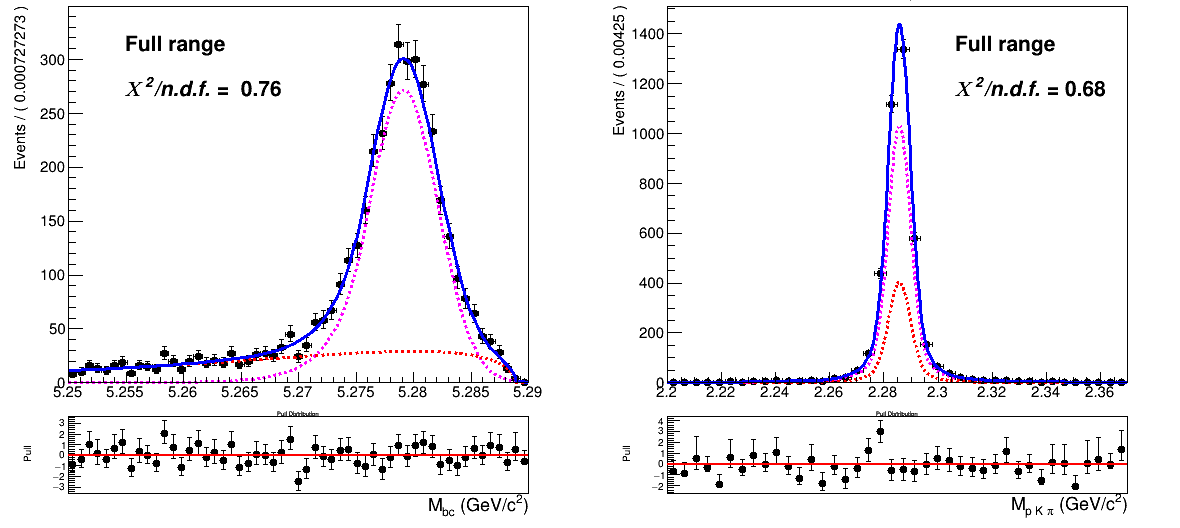
\includegraphics[width=0.75\textwidth]{04-SimultaneousFit/figs/stream0_TotalSignal_charged_corrLambdaC_2Dfit.png}}
    \caption{Two dimensional fit of Total Signal of stream 0 used to extract the expected reconstructed (corresponding to the PDF colored in magenta) and expected misreconstructed yields (corresponding to the PDF colored in red).}
    \label{fig:stream0_TotalSignal_charged_corrLambdaC_2Dfit}
    \end{figure}


\newpage

\subsection{Fit results for $B^- \rightarrow \Lambda_c^+$ decays}  

\begin{figure}[H]
\centering
{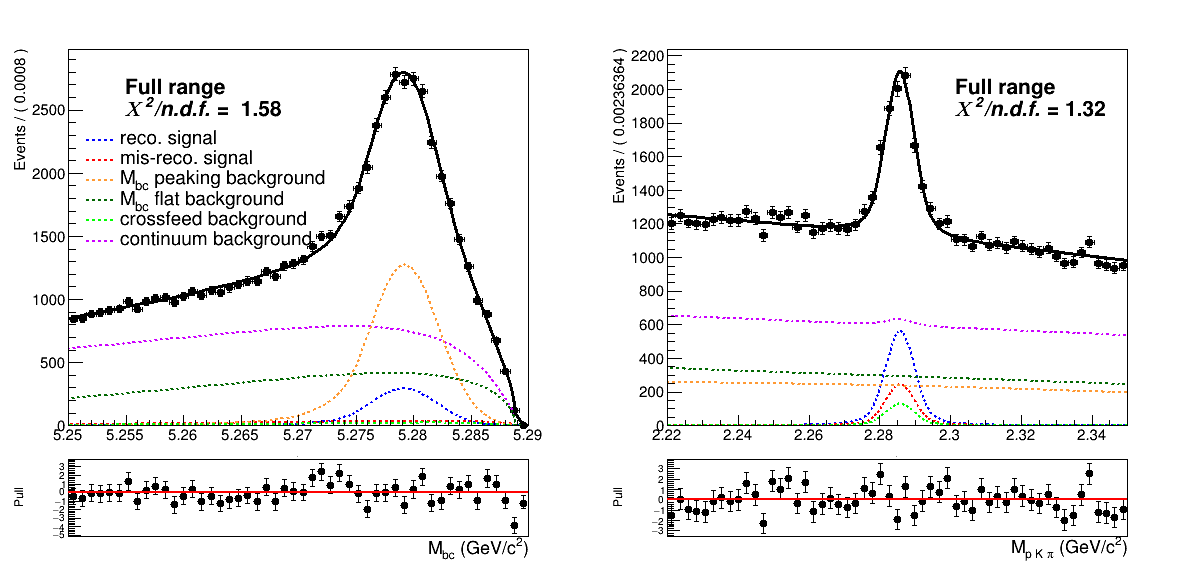
\includegraphics[width=0.90\textwidth]{04-SimultaneousFit/figs/charged_corrSample_simultaneous2DFit_stream0.png}}
\caption{Projections of the two dimensional simultaneous fit on stream 0 Monte Carlo simulated data for charged correlated decays.}
\label{fig:charged_corrSample_simultaneous2DFit_stream0}
\end{figure}

\begin{figure}[H]
    \centering
    
    {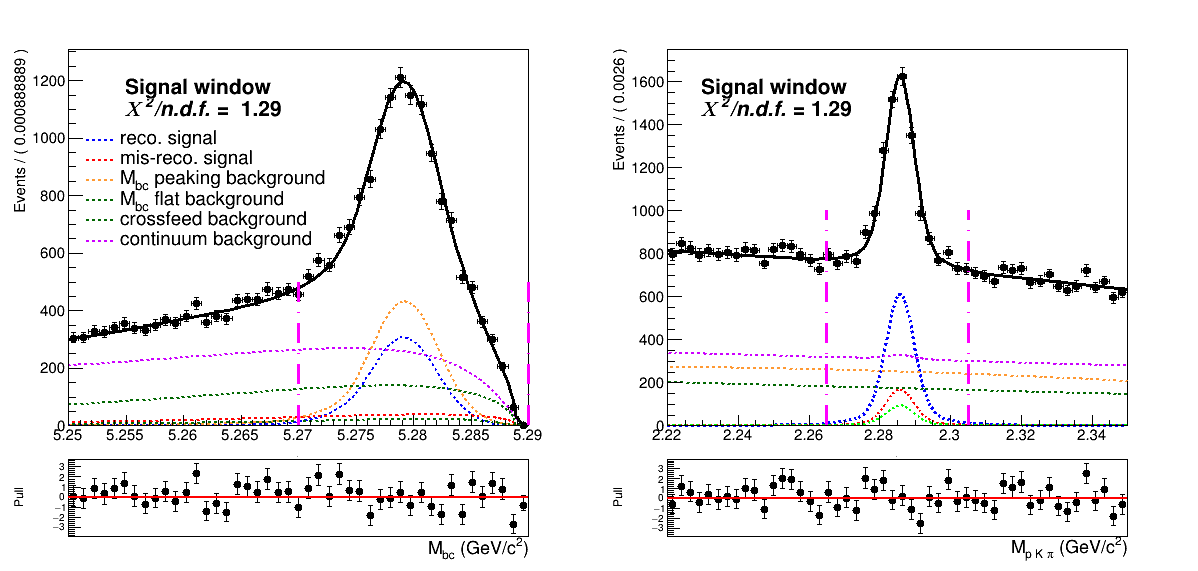
\includegraphics[width=0.90\textwidth]{04-SimultaneousFit/figs/charged_corrSignal_window_Total_2DFit_stream0.png}}
    \caption{Projections of the two dimensional simultaneous fit on stream 0 Monte Carlo simulated data for charged correlated decays(in the signal window) }
    \label{fig:charged_corrSignal_window_Total_2DFit_stream0}
    \end{figure}

\begin{table}[H]
    \centering
    \resizebox{0.99\textwidth}{!}{%
    \setlength{\tabcolsep}{8pt}
    \begin{tabular}{c c c c c c c}
    
    \toprule
     \hline
       &	\multicolumn{2}{c}{Reconstructed Signal}  & \multicolumn{2}{c}{Total Signal} &  \\
         &  fit \hspace{0.5 cm}  & expected  & fit   & MC truth &  \multicolumn{2}{c}{fit - MC truth} \\
     \midrule
     \hline
    stream 0	&	2829 $\pm$ 130 	&	2928 $\pm$ 66	&	4063 $\pm$ 157	&	4061	&  -2	&	-0.05$\%$	\\
    stream 1	&	2811 $\pm$ 137	&	2956 $\pm$ 65	&	4095 $\pm$ 161	&	4084	&  11	&	0.3$\%$	\\
    stream 2	&	2952 $\pm$ 141	&	2940 $\pm$ 65	&	4345 $\pm$ 165	&	4138	& 207	&	5.0$\%$	\\
    stream 3	&	2747 $\pm$ 134	&	2867 $\pm$ 66	&	4267 $\pm$ 160	&	4105	& 162  &   	3.9$\%$	\\
    stream 4	&	3043 $\pm$ 138	&	3017 $\pm$ 67	&	4148 $\pm$ 157	&	4176	& -28	&	-0.7$\%$	\\
    stream 5	&	2818 $\pm$ 136	&	2816 $\pm$ 65	&	3999 $\pm$ 162	&	4001	&  -2	&	-0.05$\%$	\\
    \midrule
    \hline
    sum			&	17200		&	17524	&		24917		&	24565	&	348	&	1.4$\%$	\\
    \bottomrule
    \hline
    \end{tabular}%
    }%
    \caption{Charged correlated decays: comparison of fitted and expected signal yields, fitted and truth-matched total signal for six streams of Belle generic MC when fitting the two dimensional distributions of $M_{bc}$ and $M(p K \pi)$.}
    \label{tab:SixStreams_chargedCorrLam2Dfits}
    \end{table}
    

    The yields obtained by the fit show a slight tendency of underestimation, but when comparing the sums of them with the sum of expected 
    values one can see the difference is within statistical fluctuations ( within 2$\%$). 
   \\
   The tendency of underestimation is visible in , but it is just slightly larger than $\sigma$


   \begin{figure}[H]
    \centering
    {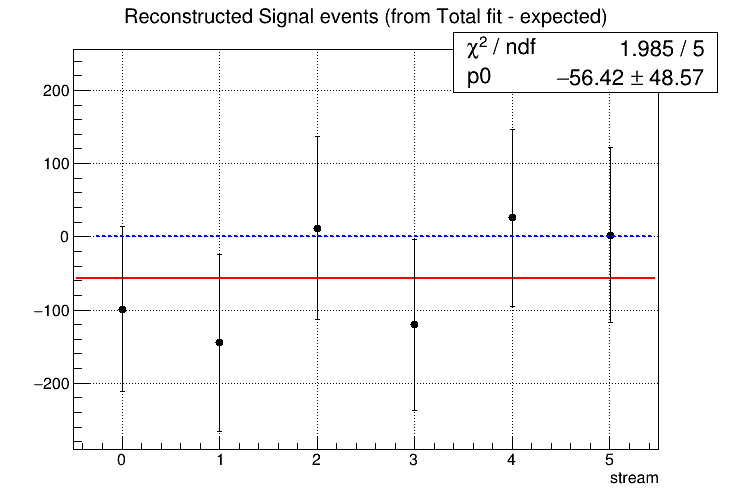
\includegraphics[width=0.70\textwidth]{04-SimultaneousFit/figs/6streamResults_chargedCorrelated_correct.png}}
    \caption{Residuals of signal yields (alias reconstructed signal, values reported in the first two columns of the above displayed table).}
    \label{fig:6streamsResults_chargedCorrelated}
    \end{figure}


\newpage    

\subsection{Fit results for $B^- \rightarrow \bar{\Lambda}_c^-$ decays}   

For the anticorrelated decays from charged $B$ mesons the slight tendency is in the opposite direction. But the distribution of residuals (see \cref{fig:6streamsResults_chargedAnticorrelated})
shows this slight overestimation is well within the statistical uncertainty.



\begin{table}[b]
    \centering
    \resizebox{0.95\textwidth}{!}{%
    \setlength{\tabcolsep}{8pt}
    \begin{tabular}{c c c c c c c}
    
    \toprule
     \hline
       &	\multicolumn{2}{c}{Reconstructed Signal}  & \multicolumn{2}{c}{Total Signal} &  \\
         &  fit \hspace{0.5 cm}  & expected  & fit   & MC truth &  \multicolumn{2}{c}{fit - MC truth} \\
     \midrule
     \hline
    stream 0	&	724 $\pm$ 64 	&	695 $\pm$ 28	&	813 $\pm$ 73	&	765	&  48	&	6.3$\%$	\\
    stream 1	&	726 $\pm$ 65	&	709 $\pm$ 29	&	802 $\pm$ 67	&	785	&  17	&	2.2$\%$	\\
    stream 2	&	788 $\pm$ 72	&	718 $\pm$ 29	&	911 $\pm$ 72	&	797	& 114	&	14.3$\%$	\\
    stream 3	&	679 $\pm$ 60	&	702 $\pm$ 29	&	768 $\pm$ 66	&	802	& -34  &   	4.2$\%$	\\
    stream 4	&	844 $\pm$ 73	&	710 $\pm$ 29	&	982 $\pm$ 73	&	785	& 197	&	25.1$\%$	\\
    stream 5	&	605 $\pm$ 63	&	675 $\pm$ 29	&	722 $\pm$ 63	&	760	&  -38	&	-5.0$\%$	\\
    \midrule
    \hline
    sum			&	4366		&	4209	&		4998		&	4694	&	304	&	6.5$\%$	\\
    \bottomrule
    \hline
    \end{tabular}%
    }%
    \caption{Charged anticorrelated decays: comparison of fitted and expected signal yields, fitted and truth-matched total signal for six streams of Belle generic MC when fitting the two dimensional distributions of $M_{bc}$ and $M(p K \pi)$.}
    \label{tab:SixStreams_chargedAntiLam2Dfits}
    \end{table}

    \begin{figure}[H]
        \centering
        {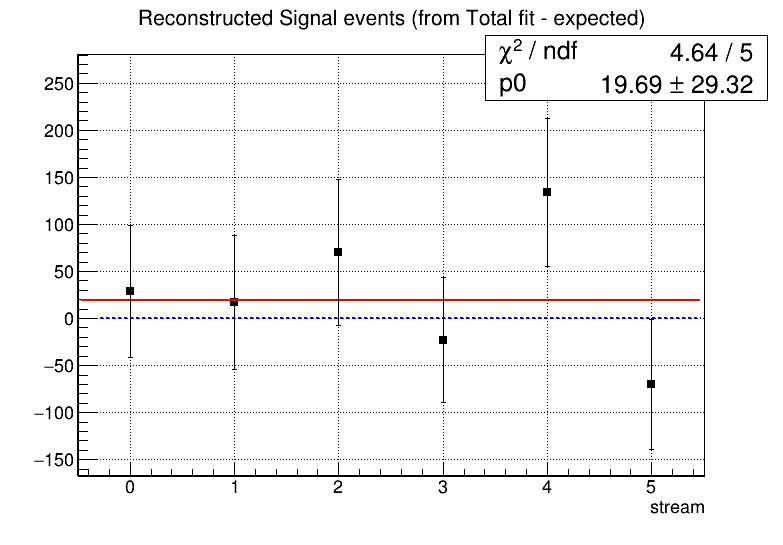
\includegraphics[width=0.70\textwidth]{04-SimultaneousFit/figs/6streamsResults_chargedAnticorrelated.png}}
        \caption{Residuals of signal yields (alias reconstructed signal, values reported in the first two columns of the above displayed table).}
        \label{fig:6streamsResults_chargedAnticorrelated}
        \end{figure}

\begin{figure}[H]
\centering
{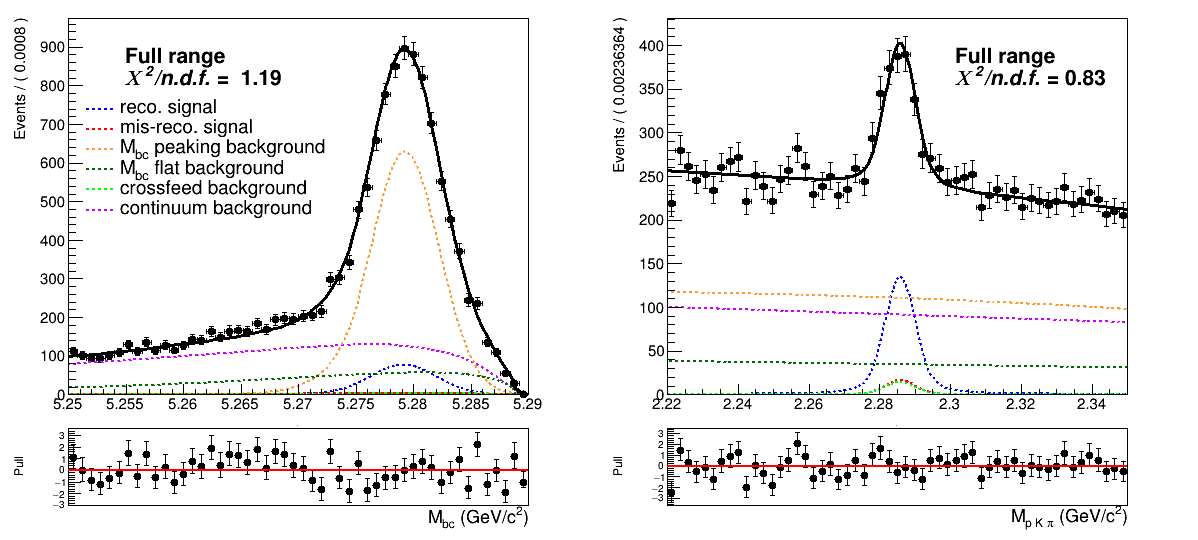
\includegraphics[width=0.90\textwidth]{04-SimultaneousFit/figs/charged_antiSample_simultaneous2DFit_stream0.png}}
\caption{Projections of the two dimensional simultaneous fit on stream 0 Monte Carlo simulated data for charged anticorrelated decays.}
\label{fig:charged_antiSample_simultaneous2DFit_stream0}
\end{figure}

\begin{figure}[H]
    \centering
    {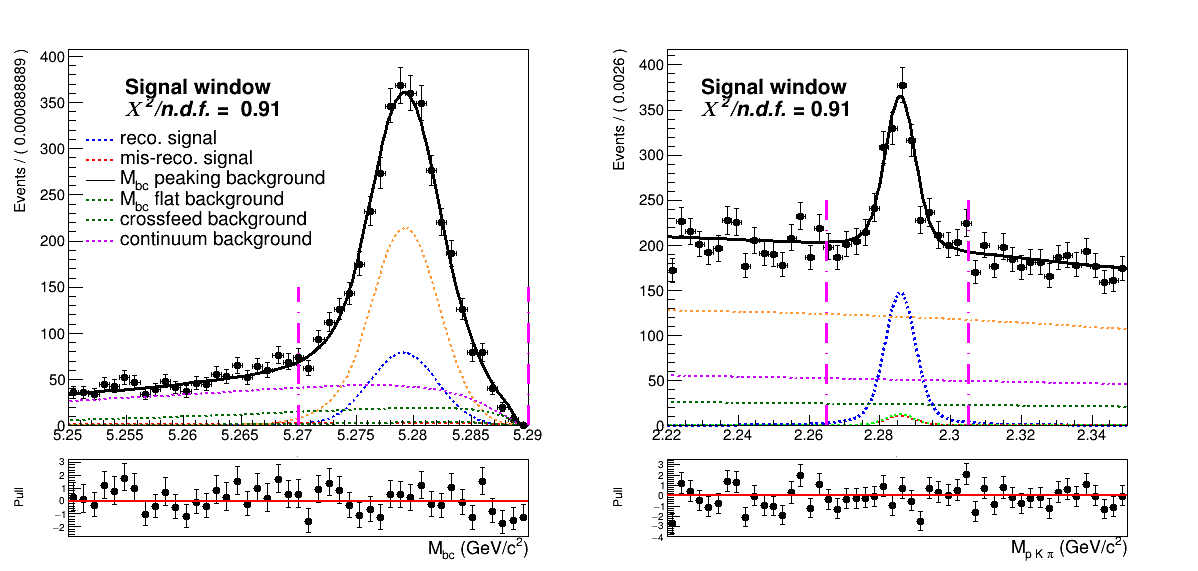
\includegraphics[width=0.90\textwidth]{04-SimultaneousFit/figs/charged_antiSignal_window_Total_2DFit_stream0.png}}
    \caption{Projections of the two dimensional simultaneous fit on stream 0 Monte Carlo simulated data for charged anticorrelated decays (in the signal window).}
    \label{fig:charged_antiSignal_window_Total_2DFit_stream0}
    \end{figure}

\newpage
\subsection{Fit results for $\bar{B^0} \rightarrow \Lambda_c^+$ decays}  
    
Also in the case of the neutral correlated one can observe a slight overestimation in the reconstructed signal yields.
The residuals (see \cref{fig:RecoSignal_streams_fit_neutralCorrLambdaC}) show that this is not so negligible: 
the significance is about 1.5$\sigma$.

\begin{table}[H]
    \centering
    \resizebox{0.95\textwidth}{!}{%
    \setlength{\tabcolsep}{8pt}
    \begin{tabular}{c c c c c c c}
    
    \toprule
     \hline
       &	\multicolumn{2}{c}{Reconstructed Signal}  & \multicolumn{2}{c}{Total Signal} &  \\
         &  fit \hspace{0.5 cm}  & expected  & fit   & MC truth &  \multicolumn{2}{c}{fit - MC truth} \\
     \midrule
     \hline
    stream 0	&	1329 $\pm$ 69 	&	1240 $\pm$ 38	&	1390 $\pm$ 70	&	1379	&  11	&	0.8$\%$	\\
    stream 1	&	1314 $\pm$ 68	&	1327 $\pm$ 38	&	1319 $\pm$ 66	&	1287	&  14	&	2.5$\%$	\\
    stream 2	&	1266 $\pm$ 68	&	1254 $\pm$ 38	&	1273 $\pm$ 65	&	1251	& 22	&	1.8$\%$	\\
    stream 3	&	1320 $\pm$ 67	&	1248 $\pm$ 38	&	1316 $\pm$ 66	&	1255	& 35  &   	4.9$\%$	\\
    stream 4	&	1227 $\pm$ 67	&	1214 $\pm$ 38	&	1300 $\pm$ 66	&	1223	&  77	&	6.3$\%$	\\
    stream 5	&	1282 $\pm$ 70	&	1233 $\pm$ 38	&	1251 $\pm$ 66	&	1246	&  5	&	0.4$\%$	\\
    \midrule
    \hline
    sum			&	7738		&	7516	&		7709		&	7525	&	140	&	1.86$\%$	\\
    \bottomrule
    \hline
    \end{tabular}%
    }%
    \caption{Comparison of fitted and expected signal yields, fitted and truth-matched total signal for six streams of Belle generic MC when fitting the two dimensional distributions of $M_{bc}$ and $M(p K \pi)$.}
    \label{tab:SixStreams_neutralCorrLam2Dfits}
    \end{table}
    
    

\begin{figure}[H]
\centering
{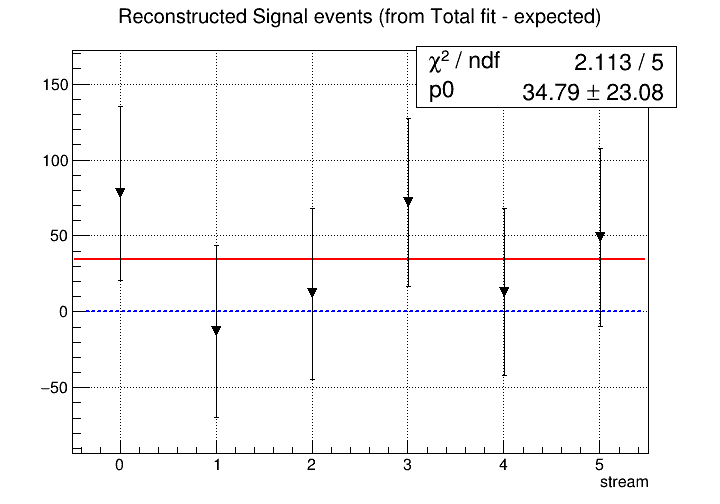
\includegraphics[width=0.70\textwidth]{04-SimultaneousFit/figs/RecoSignal_streams_fit_neutralCorrLambdaC.png}}

\caption{Residuals of signal yields for neutral correlated decays.}
        \label{fig:RecoSignal_streams_fit_neutralCorrLambdaC}
        \end{figure}    

\begin{figure}[H]
\centering
{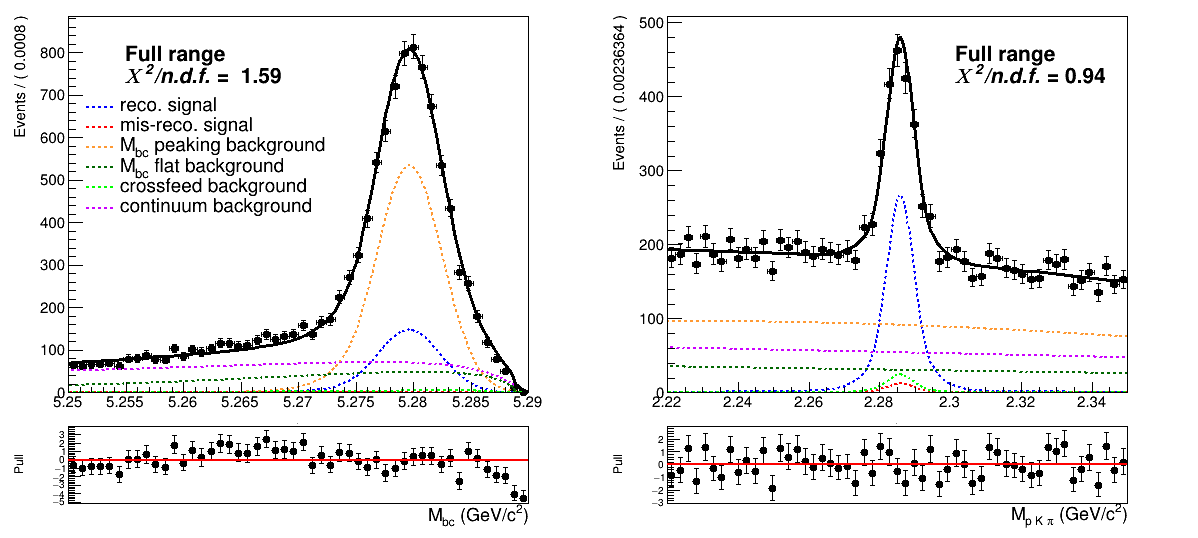
\includegraphics[width=0.90\textwidth]{04-SimultaneousFit/figs/neutral_corrSample_simultaneous2DFit_stream0.png}}
\caption{Projections of the two dimensional simultaneous fit on stream 0 Monte Carlo simulated data for neutral correlated decays.}
\label{fig:neutral_corrSample_simultaneous2DFit_stream0}
\end{figure}

\begin{figure}[H]
    \centering
    {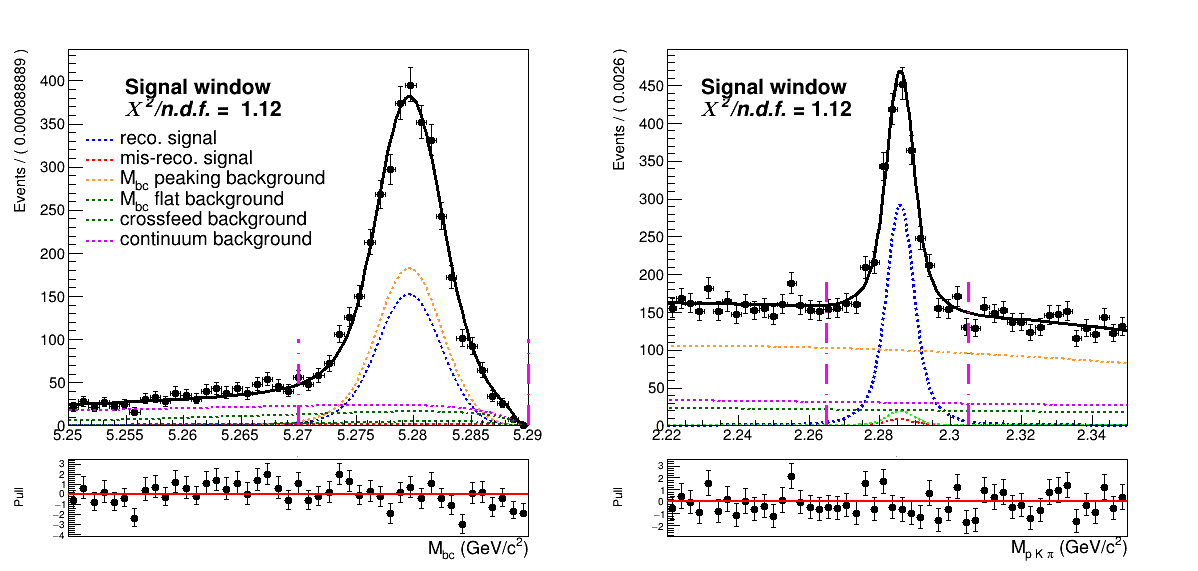
\includegraphics[width=0.90\textwidth]{04-SimultaneousFit/figs/neutral_corrSignal_window_Total_2DFit_stream0.png}}
    \caption{Projections of the two dimensional simultaneous fit on stream 0 Monte Carlo simulated data for neutral correlated decays.}
    \label{fig:neutral_corrSignal_window_Total_2DFit_stream0}
    \end{figure}



    
    \begin{figure}[H]
        \centering
        {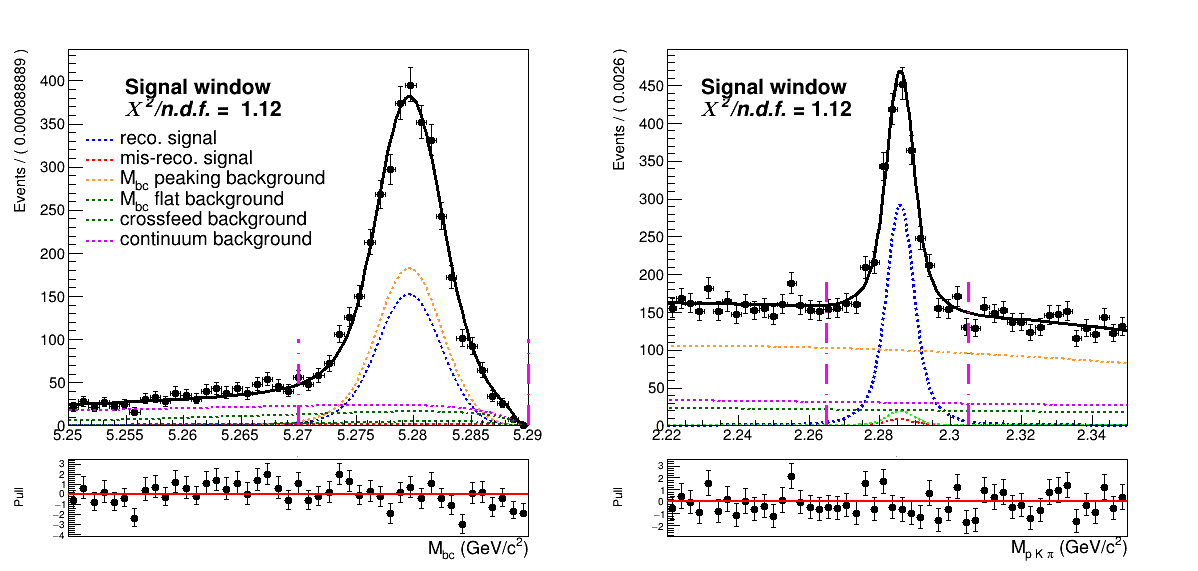
\includegraphics[width=0.90\textwidth]{04-SimultaneousFit/figs/neutral_corrSignal_window_Total_2DFit_stream0.png}}
        \caption{Projections of the two dimensional simultaneous fit on stream 0 Monte Carlo simulated data for neutral correlated decays (in the signal window).}
        \label{fig:neutral_corrSignal_window_Total_2DFit_stream0}
        \end{figure}

        
\subsection{Fit results for $\bar{B^0} \rightarrow \bar{\Lambda}_c^-$ decays} 


\begin{table}[H]
    \centering
    \resizebox{0.8\textwidth}{!}{%
    \setlength{\tabcolsep}{8pt}
    \begin{tabular}{c c c c c c c}
    
    \toprule
     \hline
       &	\multicolumn{2}{c}{Reconstructed Signal}  & \multicolumn{2}{c}{Total Signal} &  \\
         &  fit \hspace{0.5 cm}  & expected  & fit   & MC truth &  \multicolumn{2}{c}{fit - MC truth} \\
     \midrule
     \hline
    stream 0	&	567 $\pm$ 45 	&	575 $\pm$ 29	&	657 $\pm$ 45	&	668	& -11 	&	-1.6$\%$	\\
    stream 1	&	565 $\pm$ 46	&	607 $\pm$ 21	&	660 $\pm$ 47	&	687	&  -27	&	-3.9$\%$	\\
    stream 2	&	574 $\pm$ 46	&	593 $\pm$ 20	&	659 $\pm$ 45	&	639	& 20 &	3.1$\%$	\\
    stream 3	&	714 $\pm$ 49	&	596 $\pm$ 21	&	792 $\pm$ 52	&	680	& 112  &   	16.4$\%$	\\
    stream 4	&	603 $\pm$ 50	&	594 $\pm$ 21	&	693 $\pm$ 50	&	638	& 55	&	8.6$\%$	\\
    stream 5	&	589 $\pm$ 63	&	595 $\pm$ 21	&	603 $\pm$ 44	&	624	&  -21	&	3.4$\%$	\\
    \midrule
    \hline
    sum			&	3612		&	3560	&		4064		&	3936	&	170	&	4.3$\%$	\\
    \bottomrule
    \hline
    \end{tabular}%
    }%
    \caption{Neutral anticorrelated decays: comparison of fitted and expected signal yields, fitted and truth-matched total signal for six streams of Belle generic MC when fitting the two dimensional distributions of $M_{bc}$ and $M(p K \pi)$.}
    \label{tab:SixStreams_neutral_anticorrLam2Dfits}
    \end{table}

\begin{figure}
\centering
{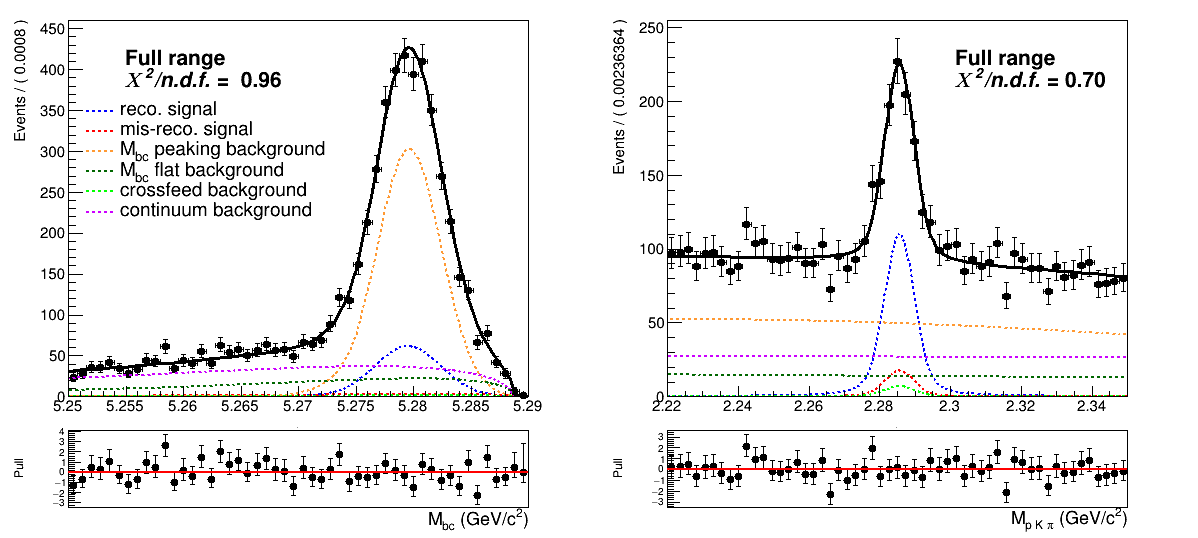
\includegraphics[width=0.83\textwidth]{04-SimultaneousFit/figs/neutral_anticorrSample_simultaneous2DFit_stream0.png}}
\caption{Projections of the two dimensional simultaneous fit on stream 0 Monte Carlo simulated data for neutral anticorrelated decays.}
\label{fig:neutral_anticorrSample_simultaneous2DFit_stream0}
\end{figure}

    \begin{figure}[H]
        \centering
        {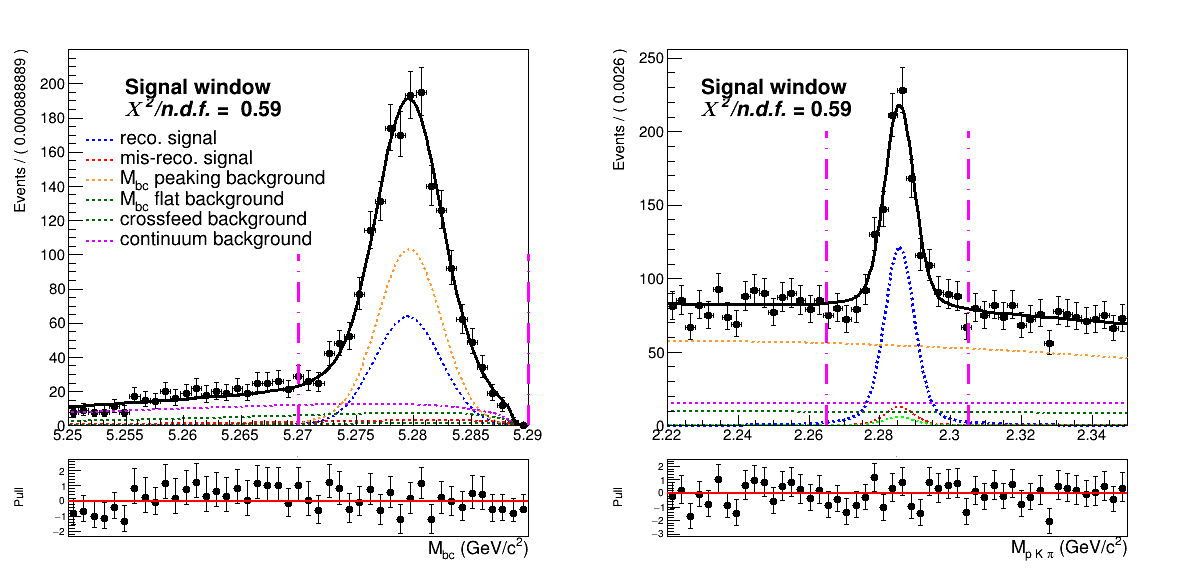
\includegraphics[width=0.90\textwidth]{04-SimultaneousFit/figs/neutral_antiSignal_window_Total_2DFit_stream0.png}}
        \caption{Projections of the two dimensional simultaneous fit on stream 0 Monte Carlo simulated data for neutral anticorrelated decays (in the signal window).}
        \label{fig:neutral_antiSignal_window_Total_2DFit_stream0}
        \end{figure}


\subsection{Fit residuals}

\cref{fig:2DsimFitresiduals} shows the residuals in each fit (stream by stream), calculated as the difference of reconstructed
signal yield in the two dimensional fit from the expected value (in the fit of the total signal events). Since the signal events are the same 
in the two fits, the resulting yields are correlated. Therefore the uncertainties on the residuals are calculated  (on a first approximation)
as: 
\begin{equation}
\sigma_{res} = \sqrt(\sigma^2_{tot} - \sigma^2_{sig})
\end{equation}




\begin{figure}
\centering
{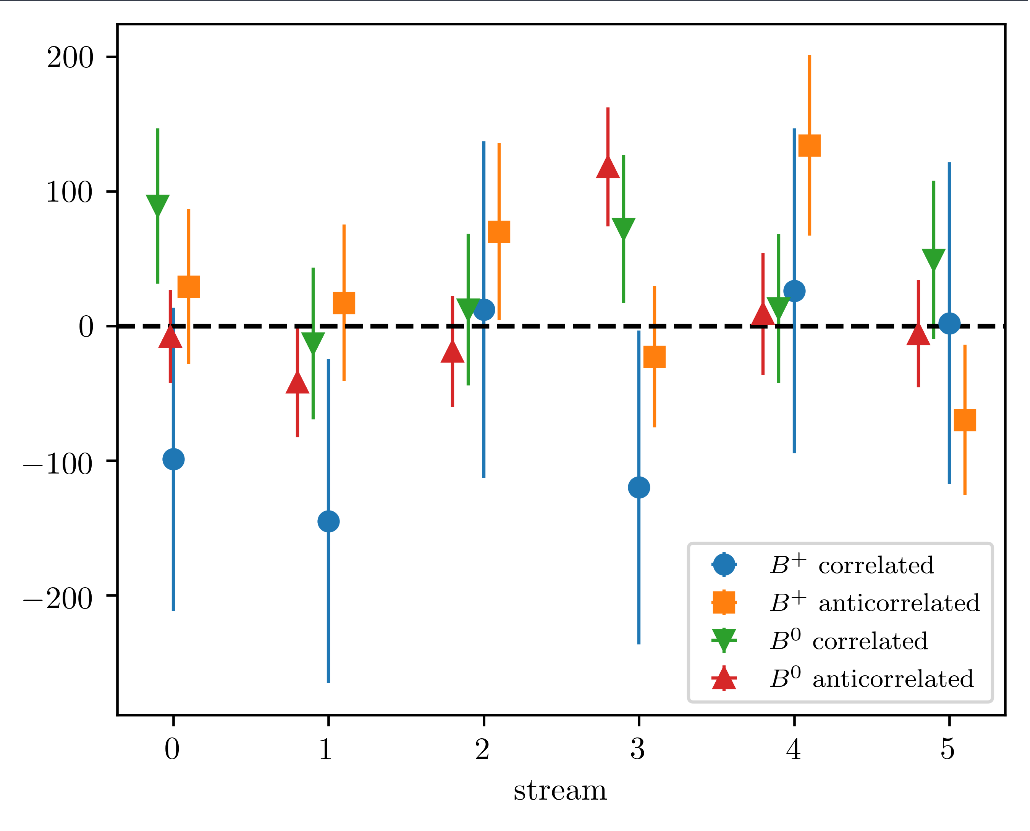
\includegraphics[width=0.85\textwidth]{04-SimultaneousFit/figs/2DsimFitresiduals.png}}
\caption{Residuals of the fitted signal yields resulting from the simultaneous 2D fit by stream and decay mode.}
\label{fig:2DsimFitresiduals}
\end{figure}

Some of the results may seem not well distributed around 0.
 

\begin{figure}[H]
    \centering
    {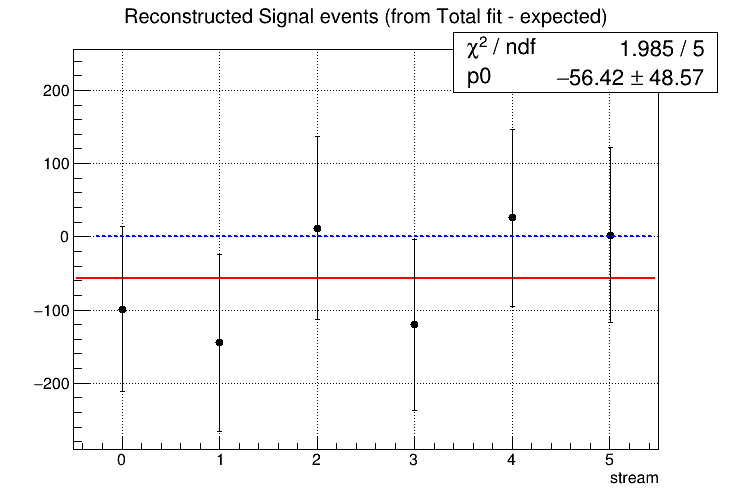
\includegraphics[width=0.85\textwidth]{04-SimultaneousFit/figs/6streamResults_chargedCorrelated_correct.png}}
    \caption{Residuals of the fitted signal yields of charged correlated decays.}
    \label{fig:6streamResults_chargedCorrelated_correct}
    \end{figure}



\newpage

\subsection{toy Monte Carlo study}

For the fit model also toy MC pseudo-experiments were performed in order to confirm the behavior of the fit setup. 
With toy MC experiments the yields, errors and the pulls of the fit are studied by generating our own pseudo-datasets, according to the MC (see plots in
3$\times 10^3$ pseudo-datasets are constructed, where each dataset was generated with the expected amount of events, 
distributed according to the Poisson distribution. Then the composition of each toy pseudo-experiment is fitted as if they were data, and
the pull-value distributions of the fit results are calculated. From the plots showing the  
 pull distributions of the fitted signal yields one can conclude that no bias is present. 
 
 

\begin{figure}[H]
    \centering
    {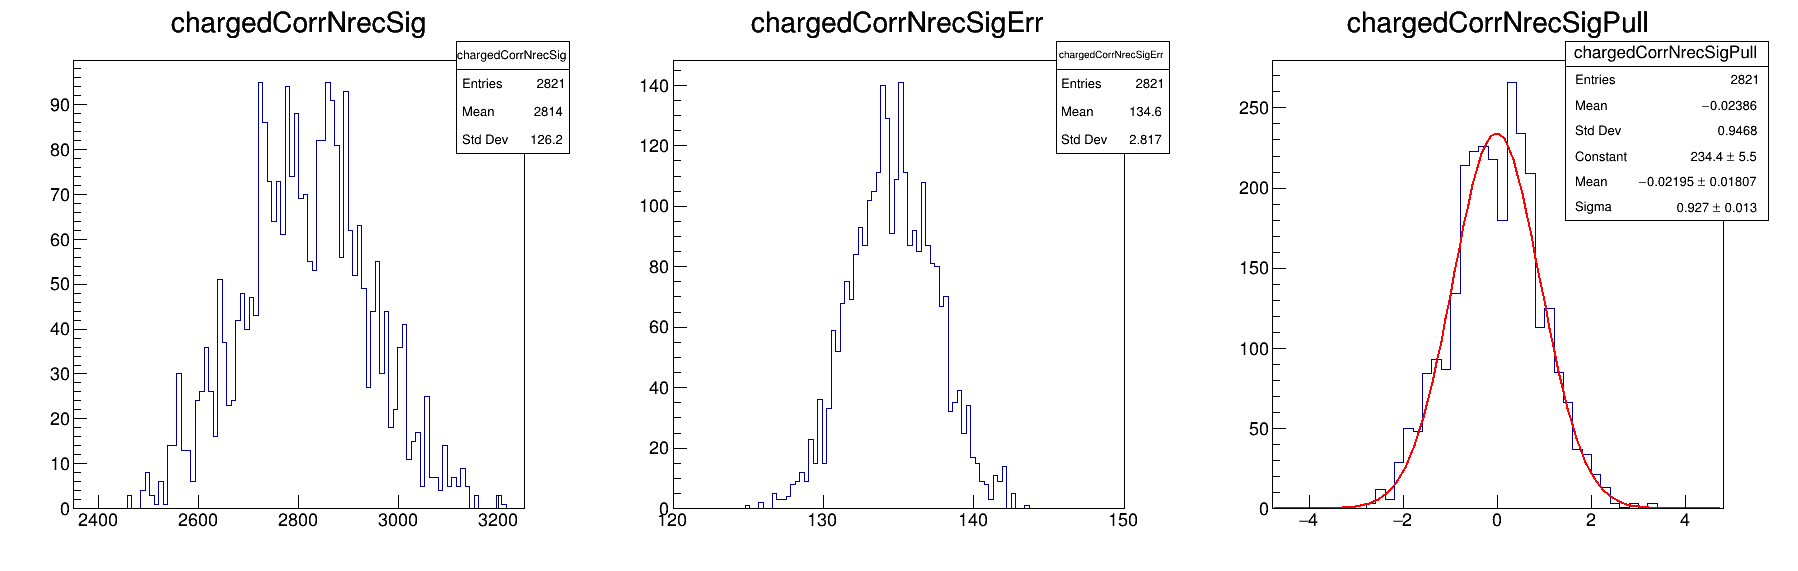
\includegraphics[width=0.85\textwidth]{04-SimultaneousFit/figs/chargedCorrNrecSigPull.png}}
    \caption{Plots showing distributions of the fitted signal yields, errors and the pull
    distribution of all pseudo-fits for the charged correlated decays.}
    \label{fig:2DchargedCorrNrecSigToys}
    \end{figure}


    \begin{figure}[H]
        \centering
        {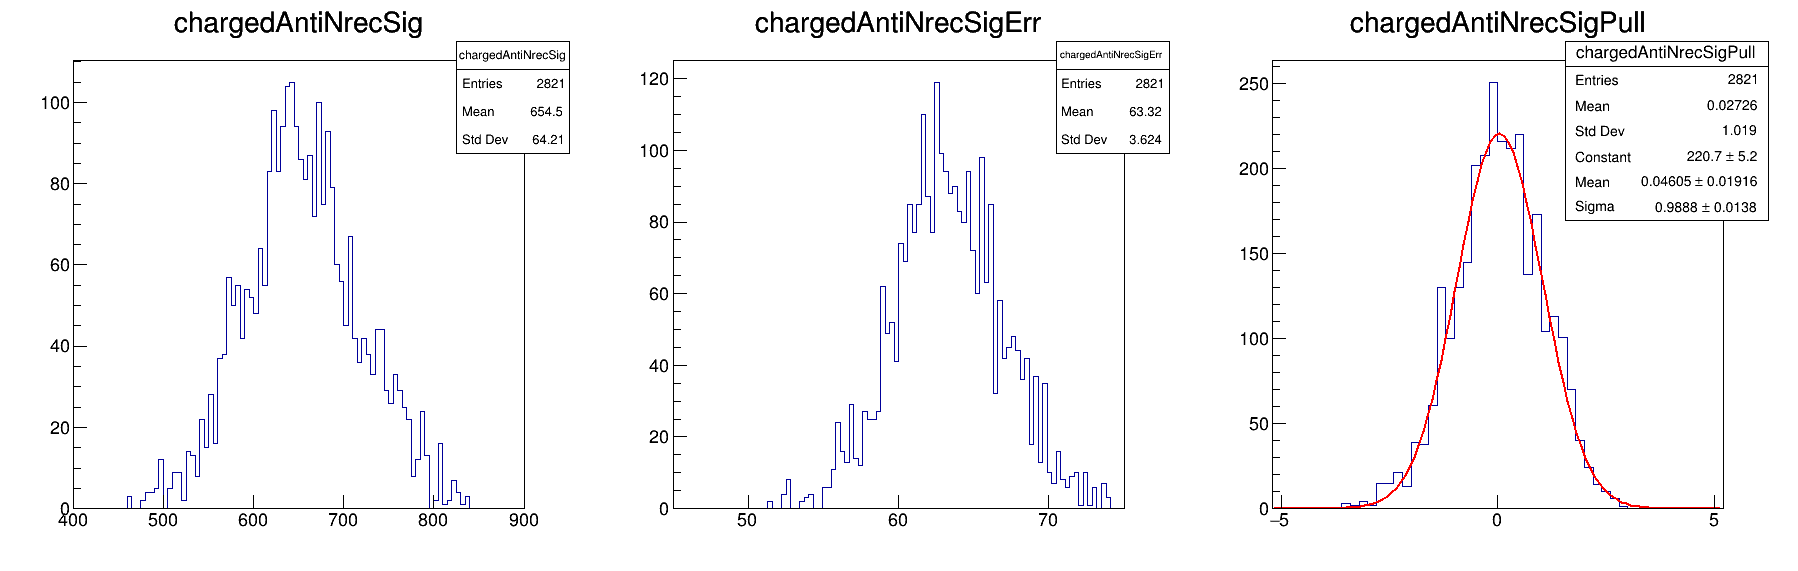
\includegraphics[width=0.85\textwidth]{04-SimultaneousFit/figs/chargedAntiNrecSigPull.png}}
        \caption{Plots showing distributions of the fitted signal yields, errors and the pull
        distribution of all pseudo-fits for the charged anticorrelated decays.}
        \label{fig:2DchargedAntiNrecSigToys}
        \end{figure}

\begin{figure}[H]
\centering
{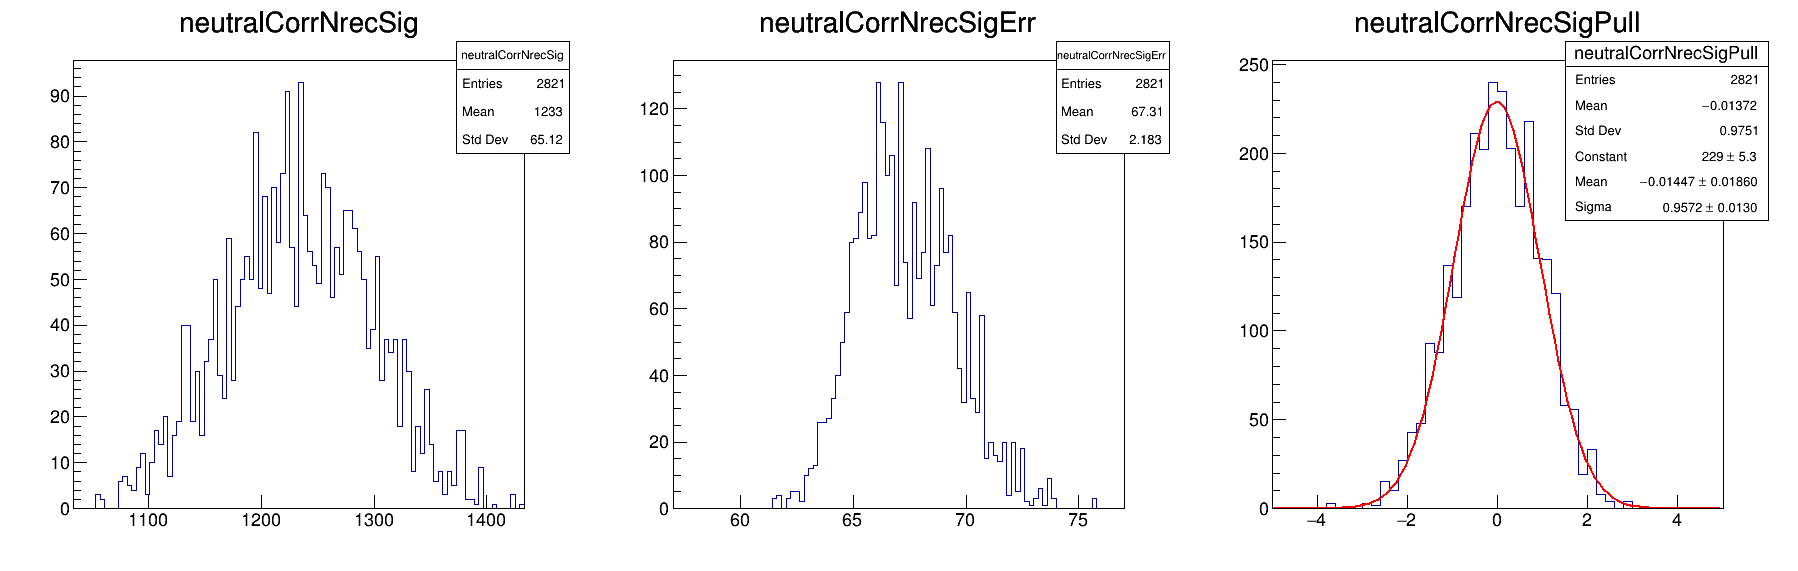
\includegraphics[width=0.85\textwidth]{04-SimultaneousFit/figs/neutralCorrNrecSigPull.png}}
\caption{Plots showing distributions of the fitted signal yields, errors and the pull
distribution of all pseudo-fits for the neutral correlated decays.}
\label{fig:2DneutralCorrNrecSigToys}
\end{figure}


\begin{figure}[H]
    \centering
    {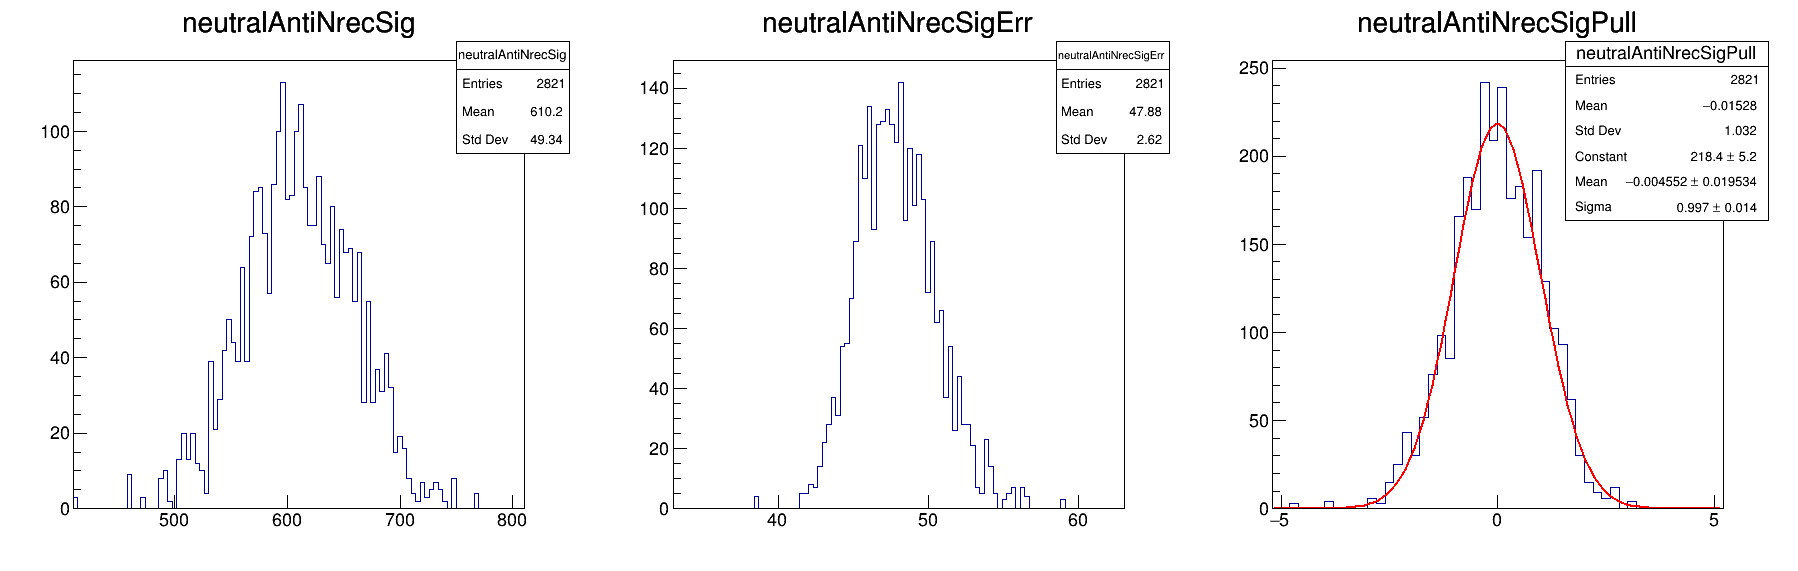
\includegraphics[width=0.85\textwidth]{04-SimultaneousFit/figs/neutralAntiNrecSigPull.png}}
    \caption{Plots showing distributions of the fitted signal yields, errors and the pull
    distribution of all pseudo-fits for the neutral anticorrelated decays.}
    \label{fig:2DneutralAntiNrecSigToys}
    \end{figure}